\chapter{Unstructured Quantum Search}
\labelChapter{unstructured_quantum_search}

\section{Introduction}
\labelSection{C2_introduction}
\lettrine[lines=3]{T}{he} canonical quantum search algorithm due to Grover~\cite{Grover_1997} provides a way to find a unique target element in an unstructured list of size $N$, provided that the specified target element exists, with high probability after $\bigO{\sqrt{N}}$ search queries, giving a quadratic advantage over a classical exhaustive search over all possible target elements, which requires $\bigO{N}$ search queries. Grover's algorithm is phrased as solving the problem of searching an unstructured list of a particular size, its applications are broad and wide-ranging, encompassing combinatorial search and optimization problems such as graph coloring problems and Boolean satisfiability problems~\cite{Mike&Ike, Dewolf_2019}. At the heart of Grover's algorithm is a quantum routine called amplitude amplification~\cite{Boyer_1998,Brassard_2002} that amplifies the amplitudes of the so-called target elements\footnote{In general, there could be more than one target element or no target element at all.} while suppressing amplitudes associated with non-target elements, thus in effect increasing the probability of measuring the target elements at end of the subroutine. It is typically phrased as follows~\cite{Brassard_2002}: Given a Boolean function $\chi : \mathbb{Z} \to \{0, 1\}$ such that one or more $x$ satisfy $\chi(x)=1$, there exists a quantum subroutine $\mathcal{A}$ that makes no use of intermediate measurements and has probability $p$ of finding a $\ket{x}$, when applied to $\ket{\textbf{0}}$. Then $\bigO{1/p}$ applications of $\mathcal{A}$ and $\mathcal{A}^{-1}$ suffice to produce the measurement outcome(s) $x$ with probability greater than half, if the applications of $\mathcal{A}$ and $\mathcal{A}^{-1}$ are followed by an appropriate measurement\footnote{As we will see later that the canonical quantum search algorithm due to Grover may be taken to be the special case of quantum amplitude amplification, where ${\mathcal{A}=H^{\otimes n}}$, such that ${p = 1/\sqrt{N}}$ (\ie ${\mathcal{A}}$ prepares an equal superposition of all possible outcomes), and the promise that there is one unique target element $s$, where ${\chi(s)=1}$.}. 

\bigskip
\noindent
There is a large body of experimental work that exists demonstrating the realization of instances of Grover's algorithm for $N=4$ on two qubits on sundry quantum architectures. The pioneering work was demonstrated on a liquid-state \gls{NMR} based quantum architecture, successfully verifying that the algorithm can find a specified target item with near-certainty in a single step of the algorithm, although in a non-programmable and non-scalable manner~\cite{Chuang_1998}. One of the very first instances of Grover's algorithm was done on a trapped-ion system~\cite{Brickman_2005}, with the ability to arbitrary specify any of the $N=4$ as a target element, and subsequently find it with one single step of the algorithm. Technological improvements over the years made similar programmable demonstrations (promises of scalability) possible~\cite{DiCarlo_2009}. The next instance of Grover's algorithm is on three qubits for a search space of $N=8$ elements; the only three-qubit experimental demonstrations of Grover's algorithm are due to Vandersypen~\etal~\cite{Vandersypen_2000} on a liquid \acs{NMR} architecture and a complete implementation (with the ability to find arbitrarily specified target elements in a programmable way) is due to Figgat~\etal~\cite{Figgatt_2017} on a trapped-ion system. At the time that the author writes this thesis, there is no complete four-qubit experimental demonstration of Grover's algorithm in its canonical form.

\clearpage
\noindent
The standard construction of the algorithm has been proven to be optimal in the number of search queries (steps)~\cite{Bennett_1997,Boyer_1998,Zalka_1999}. However, in actuality, each of these steps are broken down into intermediary subroutines. In particular, for \acs{NISQ} processors, the intermediary subroutines are further broken down into atomic operations. Such atomic (unitary) operations constitute a finite gate set called a universal gate set~\cite{Dawson_2005} for which any unitary operation can be approximated in terms of a finite set of gates from a universal gate set. In the instance of superconducting qubit based architectures, the universal gate set is realized with a set of single-qubit gates along with a high-fidelity two-qubit entangling gate~\cite{Kjaergaard_2020}. \acs{NISQ} processors are severely limited by the debilitating effects of decoherence, that limit the time over which a computation can remain fully coherent, thus there is an upper limit on the number of operations over a set of qubits that can be in a circuit mapped to a physical processor and guarantee a reliable result at the end of the computation. As it stands, standard constructions of the algorithm on four or more qubits present a sizeable challenge on \acs{NISQ} processors. 

\bigskip
\noindent
One of the intermediary subroutines of the algorithm is the so-called global Grover iterate, which constitutes the most resource intensive part of the algorithm in terms of two-qubit gate count. The global Grover iterate for the standard algorithm on $n$-qubits consists of one or more $n$-qubit Toffoli gate (modulo single gates). For $n\geq 4$ the exact controlled-NOT count for a $n$-qubit Toffoli without auxiliary of qubits is unknown~\cite{Shende_2008}. Additionally, to guarantee close to sure success of finding the target element(s), the global Grover iterate is repeated roughly $\left\lfloor {c\sqrt{N}} \right\rfloor$ times (for some positive constant $c$), which presents a considerable handicap for its physical implementation. In our preliminary tests of the standard construction of Grover's algorithm on four qubits, we found that the output probability distribution is indistinguishable from a uniform noise on the IBM quantum processors.

\bigskip
\noindent
Apart from the standard construction, there are other variants of Grover's algorithm that trade accuracy in various ways for a reduction in the number of search queries, making them suitable for small-scale implementation on \acs{NISQ} processors. For instance, it has been shown that one may stop short of $\left\lfloor {c\sqrt{N}} \right\rfloor$ search queries and still guarantee a high probability of success~\cite{Boyer_1998}, with the downside that we may have to repeat the algorithm in case of failure. Other variants, the canonical variant being due to Grover and Radhakrishnan~\cite{Grover_2005, Korepin_2006a}, modifies the Grover iterates to search for a subspace of possible elements to which the target element belongs, rather than the target element itself. This may be thought of as finding the first $n-m$ bits, for some $m$, of the target element instead of all the bits of the target element. By way of combining local and/or global Grover iterates, it is possible to reduce the number of search queries at the expense of accuracy. Here, the choice of the sequence of local and/or global Grover iterates, and the size of the local Grover iterates ($n-m$) is of practical interest in maximizing the success probability with the least number of search queries, and hence a reduced two-qubit gate count. In particular instances, local Grover iterates can be applied to the full search problem with appropriate choices for $m$. There is a large corpus of work studying the optimal sequences of local and/or global Grover iterates~\cite{Korepin_2005,Korepin_2006,Choi_2006,Korepin_2006a,Korepin_2006b}, and a configuration that has with several local Grover iterates sandwiched between one global iterate on one side and several global iterates on another has been shown to be optimal. 

\clearpage
\noindent
During the period over which this part of the thesis was conducted, several important results were published in succession~\cite{Zhang_2020,Wang_2020,Satoh_2020,Gwinner_2020,Brianski_2021,Zhang_2021} that addressed many of the questions, aims and objectives we initially had towards this particular research topic, which had the overriding imperative of reducing the resources used by algorithm, making it suitable for implementation on \acs{NISQ} devices, hence this chapter will mainly consist of a survey of these results. We also present two marginal results of our own in this chapter, the first of which is an improvement in the success probabilities of the implementation in~\cite{Satoh_2020} by way of a further iteration using a local Grover iterate. Alas, the improvements in the results are most probably indicative of the improvement in the quality of the devices used rather than anything particular to our construction as it uses more controlled-NOT gates in comparison. The second result is related to a measurement-based three-qubit implementation of Grover's algorithm, and we also present results of implementing a measurement-based controlled-controlled-$Z$ (equivalent to three-qubit Toffoli gate), which is an important subroutine in the algorithm. The results are unfortunately negative, as the measurement-based controlled-controlled-$Z$ necessarily requires a graph state of ten qubits with twelve edge connections (controlled-$Z$ gates between nodes), which cannot be further reduced by edge local complementation. For these reasons, it is out of reach for current \acs{NISQ} devices.

\section{Background}
\labelSection{C2_background}

\subsection{Canonical construction of Grover's algorithm}
\labelSection{C2_canonical_construction_of_grovers_algorithm}

We begin by reviewing the standard construction of the algorithm in the circuit model of quantum computation, closely following Refs.~\cite{Grover_1997, Mike&Ike, Dewolf_2019}. The Grover's algorithm provides a way to solve the following dilemma:


\bigskip
\noindent
On one faithful day, you happen to have locked yourself out of the laboratory and for some reason urgently need to access to your laboratory\footnote{Based on a true story.}. To worsen your woes, you realize that you completely forgot the lock combination, but luckily you happen to recall that the lock in question uses a lock-mechanism as the one shown in~\refFigureOnly{switches}; it has $n$-switches each of which has an \enquote{on} and \enquote{off} setting, and the lock combination that unlocks your laboratory is some unique configuration $s$ of the $n$ switches, with each being either set to either \enquote{on} or \enquote{off}.

\begin{figure}[h]
    \centering
	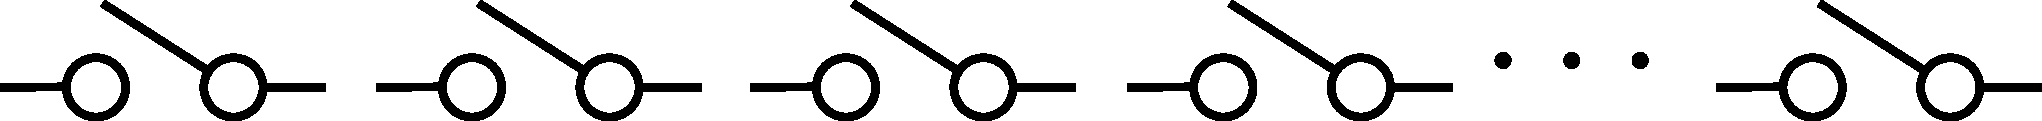
\includegraphics[width=0.75\linewidth]{switches}
	\caption[A configuration of $n$ binary switches where some configuration of the switches is denoted a winning configuration, as an example to illustrate of the search problem Grover's algorithm tries to solve.][-10pt]{A configuration of $n$ binary switches where some configuration of the switches is denoted a winning configuration, as an example to illustrate the search problem Grover's algorithm tries to solve.} 
	\labelFigure{switches}
\end{figure}

\noindent
If you don't have any prior knowledge of the configuration $s$, the best you can do is to simply employ a random guess and check strategy, \ie you might try the combination shown in~\refFigureOnly{switches_comb} and check if the lock opens.

\begin{figure}[h]
    \centering
	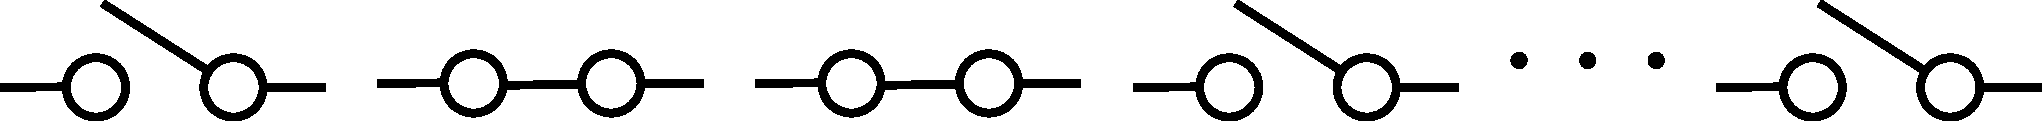
\includegraphics[width=0.75\linewidth]{switches_comb}
	\caption[An example configuration of the $n$ binary switches where two of the switches are in the on state and rest are in the off state.]{An example configuration of the $n$ binary switches where two of the switches are in the on state and rest are in the off state.}
	\labelFigure{switches_comb}
\end{figure}

\noindent
If this is the best you can do, in the worst-case scenario you should expect to try all possible combinations, of which there are $N=2^n$, until you find $s$, thus the worst-case behaviour scales linearly with $N$, $\bigO{N}$. 

\clearpage
\noindent
We can rephrase the above problem more concretely; assume we have the Boolean function $\chi: \{0, 1, \ldots, N-1\} \to \{0,1\}$ such that

\begin{align}
\labelEquation{check_function}
\chi(x) =
	\begin{dcases}
		1 & x=s \\
		0 & x\neq s
	\end{dcases},
\end{align}

\noindent 
for some unknown $s$. We refer to $s$ as a target element. The above problem can be phrased as finding the unknown $s$ by querying the above Boolean function, with some input $x$ and check if $\chi(x) = 1$.

\bigskip
\noindent
On a quantum computer, we can do slightly better than $\bigO{N}$ for the above. We assume here that the size of the search problem is a power of $2$, $N=2^n$ for $n \in \mathbb{N}$. We can thus realize the entire search space for a particular $N$ on $n=\log{(N)}$ qubits~\footnote{All logarithms $\log(\cdot)$ are taken base $2$ unless state otherwise. $\ln(\cdot)$ is reserved for $\log_{e}$}. One of the first clever tricks is to represent the effect of the Boolean function $\chi$ to indicate whether a particular input is a target element as a unitary transformation $U_{\chi}$, which acts on basis states $\ket{x}$ like so,

\begin{align}
U_{\chi}: \ket{x} \to (-1)^{\chi(x)} \ket{x}.
\end{align}

\noindent
Observe for all $x \neq s$, the above unitary transformation acts trivially on the corresponding basis state $\ket{x}$, and for $x = s$, the corresponding basis state acquires a negative phase; the unitary $U_{\chi}$ is often called a phase oracle. $U_{\chi}$ may be written explicitly as,

\begin{align}
	\labelEquation{phase_oracle}
	U_{\chi} = \mathds{1} - 2\op{s}.
\end{align}

\noindent
The algorithm starts with an $n$-qubit state $\ket{0}^{\otimes n}$ and prepares an equal superposition of all basis states, by applying a Hadamard transformation on each qubit,  $H^{\otimes n}$

\begin{align}
	\labelEquation{equal_superpos}
	\ket{\psi} = H^{\otimes n} \ket{0}^{\otimes n} = \frac{1}{\sqrt{N}}\displaystyle\sum_{x=0}^{N-1}\ket{x}.
\end{align}

\noindent
It is useful to write the above state in a different basis. If there are $t$ target elements (and $N-t$ non-target elements), then define $\ket{x_{\perp}}$ and $\ket{x_{//}}$ as such 

\begin{align}
	\ket{x_{\perp}} &= \frac{1}{\sqrt{N-t}}\displaystyle\sum_{x \neq s}\ket{x}, \nonumber \\ 
	\ket{x_{//}} &= \frac{1}{\sqrt{t}}\displaystyle\sum_{x = s}\ket{x},
\end{align}


\noindent
we can rewrite $\ket{\psi}$ as

\begin{align}
	\labelEquation{sol_basis}
	\ket{\psi} = \frac{\sqrt{N-t}}{\sqrt{N}}\ket{x_{\perp}} + \frac{\sqrt{t}}{\sqrt{N}} \ket{x_{//}},
\end{align}

\noindent
We can further adopt the parametrization

\begin{align}
	\theta &= \arcsine{\sqrt{\frac{t}{N}}}, \nonumber \\
	\cos{(\theta)} &= \sqrt{\frac{N-t}{N}}, \nonumber \\
	\sin{(\theta)} &= \sqrt{\frac{t}{N}},
\end{align}

\noindent
for which we can further rewrite~\refEquationOnly{sol_basis} as

\begin{align}
	\labelEquation{angle_basis}
	\ket{\psi} = \cos{(\theta)}\ket{x_{\perp}} + \sin{(\theta)}\ket{x_{//}}.
\end{align}

\noindent
Applying $U_f$ to the above state yields

\begin{align}
	\labelEquation{oracle_app}
	U_{\chi} \ket{\psi} = \cos(\theta)\ket{x_{\perp}} - \sin{(\theta)}\ket{x_{//}}.
\end{align}

\noindent
Another clever trick in Grover's algorithm is an application of another unitary transformation $D$; defined similarly to~\refEquationOnly{phase_oracle}

\begin{align}
	D &= H^{\otimes n} (2\op{0}^{\otimes n} - \mathds{1}) H^{\otimes n}, \nonumber \\
	D &= 2\op{\psi} - \mathds{1}.
\end{align}

\noindent
The above unitary transformation is often called a global diffuser operator. Expanding $D$ in terms of the basis $\{\ket{x_{\perp}}, \ket{x_{//}}\}$, we get to the expression

\begin{align}
	D &= 2\cos^2{(\theta)} \ket{x_{\perp}}\bra{x_{\perp}}  + 2\sin^2{(\theta)}\ket{x_{//}}\bra{x_{//}} \nonumber \\
	&\quad + \sin{(2\theta)}\ket{x_{\perp}}\bra{x_{//}} + \sin{(2\theta)}\ket{x_{//}}\bra{x_{\perp}} - \mathds{1}.
\end{align}

\noindent
We apply $D$ to~\refEquationOnly{oracle_app}, after trigonometric and algebraic gymnastics we arrive at

\begin{align}
	\labelEquation{so2_mat}
	D U_{\chi} \ket{\psi} &= (\cos{2\theta}\cos{\theta} - \sin{2\theta}\sin{\theta})\ket{x_{\perp}} \nonumber \\
					 &\quad + (\sin{2\theta}\cos{\theta} + \cos{2\theta}\sin{\theta})\ket{x_{//}}, \nonumber  \\
					 &= \cos{3\theta}\ket{x_{\perp}} + \sin{3\theta}\ket{x_{//}}.
\end{align}

\noindent
The full $D U_{\chi}$ has a geometric interpretation; the state $\ket{\psi}$ is a vector in a $2$-dimensional Euclidean space spanned by $\ket{x_{\perp}}$ and $\ket{x_{//}}$, initially angled at $\theta$ with respect to $\ket{x_{\perp}}$. $U_{\chi}$ reflects the vector $\ket{\psi}$ about the $\ket{x_{\perp}}$ axis, \ie $\theta \mapsto - \theta$; the angle between $\ket{\psi}$ and $U_{\chi}\ket{\psi}$ at this point is $2\theta$. $D$ finally reflects $U_{\chi}\ket{\psi}$ about the $\ket{\psi}$ axis; the angle between $\ket{x_{\perp}}$ and $D U_{\chi}\ket{\psi}$ is $3\theta$; see figure below.

\begin{figure}[h]
    \centering
	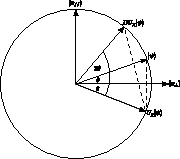
\includegraphics[width=0.60\linewidth]{grover}
	\caption[The geometric interpretation of a single Grover iterate.]{The geometric interpretation of  a single Grover iterate; the uniform superposition state $\ket{\psi}$ starts at an angle $\theta$ with respect to the axis $\ket{x_{\perp}}$, the action of the phase oracle $U_{\chi}$ reflects $\ket{\psi}$ about the axis $\ket{x_{\perp}}$. Likewise, the action of the diffuser operator is to reflect $U_{\chi}\ket{x_{\perp}}$ about the axis $\ket{\psi}$ to get $D U_{\chi}\ket{x_{\perp}}$.}
	\labelFigure{grover_iterate}
\end{figure}

\clearpage
\noindent
Looking at~\refEquationOnly{so2_mat}, we can conveniently write the action of $D U_{\chi}$ on the basis states $\{\ket{x_{\perp}}, \ket{x_{//}}\}$ as 

\begin{align}
	D U_{\chi} = \mqty(\cos{(2\theta)} & -\sin{(2\theta)} \\ \sin{(2\theta)} & \cos{(2\theta)}),
\end{align}

\noindent
that is, $D U_{\chi}$ is an element of the special orthogonal group $SO(2)$, the group of rotations in two dimensions. The unitary operator $G = D U_{\chi}$ is called the global Grover iterate. Rotating by an angle $\theta$ around a point $k$ times is equivalent to a single rotation by an angle $k\theta$. From this, it is easy to see that $k$ applications of $G$ give

\begin{align}
	G^{k} \ket{\psi} = \cos{((2k + 1)\theta)}\ket{x_{\perp}} + \sin{((2k+1)\theta)}\ket{x_{//}}.
\end{align}

\noindent
Another useful visualization aid for gaining intuition about the Grover iterate is look to at its effect at the level of the amplitudes of the state in~\refEquationOnly{equal_superpos}. Consider the case where there is one unique target element; as we have seen the amplitude of the target element $\ket{s}$ acquires a negative phase under the action of unitary operator $U_{\chi}$ while the other amplitudes are left unaltered, hence applying $U_{\chi}$ to~\refEquationOnly{equal_superpos} gives

\begin{align}
	\labelEquation{oracle_action}
	U_{\chi}\ket{\psi} = \frac{1}{\sqrt{N}}\left(-\ket{s} + \displaystyle\sum_{x\neq s} \ket{x}\right).
\end{align}

\noindent
It is not to hard to show that the action of the diffuser operator $D$ on a general $n$-qubit state ~$\ket{\varphi} =\sum_{x=0}^{N-1}\alpha_x\ket{x}$ is given by

\begin{align}
	\labelEquation{diffuser_action}
	D \ket{\varphi} = \displaystyle\sum_{x=0}^{N-1}(2\ev{\alpha} - \alpha_x)\ket{x},
\end{align}

\noindent
where $\ev{\alpha} = \sum_{x=0}^{N-1}\alpha_x / N$ is the average value of the amplitudes~\footnote{The action of the diffuser operator $D$ on the amplitudes of a general state is often called inversion about the average for this reason, since $\alpha_x \to 2\ev{\alpha} - \alpha_x$ for each amplitude $\alpha_x$ associated with a computational basis state $\ket{x}$.}. Hence, when we apply $D$ to $U_{\chi}\ket{\psi}$ in~\refEquationOnly{oracle_action} we obtain the following expression

\begin{align}
	D U_{\chi} \ket{\psi} &= \left(\frac{2(N-2)}{\sqrt{N}N} + \frac{1}{\sqrt{N}}\right)\ket{s} + \left(\frac{2(N-2)}{\sqrt{N}N} - \frac{1}{\sqrt{N}}\right)\displaystyle\sum_{x \neq s}\ket{x}, \nonumber \\
	&= \frac{3N - 4}{\sqrt{N}N}\ket{s} + \frac{N-4}{\sqrt{N}N}\displaystyle\sum_{x \neq s}\ket{x},
\end{align}

\noindent
since $\ev{\alpha} = (N-2)/\sqrt{N}N$; clearly, $3N - 4 > N- 4$. We see that the action of $D U_{\chi}$ is to increase the amplitude associated with the target element $\ket{s}$ while decreasing the amplitudes of the non-target elements (see~\refFigureOnly{amplitude_ampl}). For this reason, the process bears the name amplitude amplification.

\bigskip
\noindent
How many applications $k$ of the global Grover iterate should be applied to guarantee close to unity probability of observing the target element(s) $\ket{x_{//}}$ when we perform an appropriate measurement? Looking at~\refFigureOnly{grover_iterate}, we see that if we do not perform enough iterates we might undershoot and fall short of reaching $\ket{x_{//}}$. More worryingly, we might overshoot past $\ket{x_{//}}$, running the risk of having additional iterations for a clockwise round trip to cycle back close to $\ket{x_{//}}$. 

\clearpage
\begin{figure}[t]
	\subfloat[]
	{
		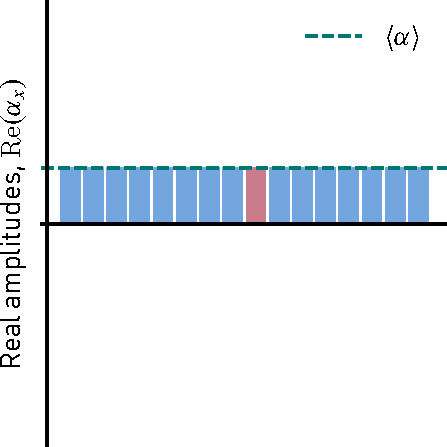
\includegraphics[width=0.33\textwidth]{grover_iter0}
	}
	\subfloat[]
	{
		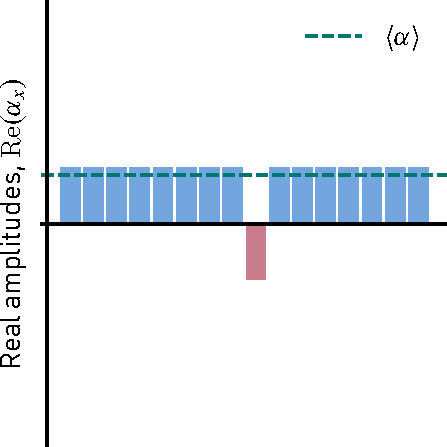
\includegraphics[width=0.33\textwidth]{grover_iter1}
	}
	\subfloat[]
	{
		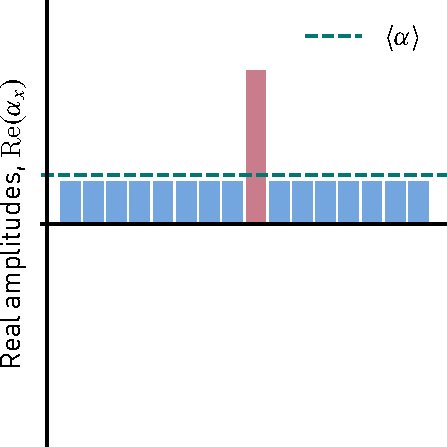
\includegraphics[width=0.33\textwidth]{grover_iter2}
	}
	\caption[The action of a single Grover iterate on the level of the amplitudes for a search space of size ${N=2^4=16}$, where we guaranteed that there is a unique target element.]{The action of a single Grover iterate on the level of the amplitudes for a search space of size ${N=2^4=16}$, when we guaranteed that there is a unique target element. \textbf{(a)} We begin with the uniform superposition state $\ket{\psi}$, the amplitude of the target state is indicated in red while the non-target elements are indicated in blue. \textbf{(b)} After applying the phase oracle, the amplitude of the target element (indicated in red) acquires a relative negative sign. \textbf{(c)} The action of the diffuser operator is to invert all amplitudes about the average amplitude $\ev{\alpha}$. Hence, non-negative amplitudes decrease while negative amplitudes increase; amplifying the amplitude of the target element.}
	\labelFigure{amplitude_ampl}
\end{figure}

\noindent
The probability of measuring $\ket{x_{//}}$ is given by

\begin{align}
	\labelEquation{prob}
	P_k = \abs{\bra{x_{//}}G^{k}\ket{\psi}}^2 = \sin{((2k+1)\theta)}^2.
\end{align}

\noindent
For a particular $\tilde{k}$, we want $P_{\tilde{k}}$ to be close to $1$, that is $\sin{((2\tilde{k}+1)\theta)}^2 \simeq 1$. From elementary trigonometry, we know that $\sin{(\phi)} = 1$ if $\phi = \pi/2$, then it must be that $(2\tilde{k}+1)\theta=\pi/2$, giving $\tilde{k} = \pi/4\theta - \frac{1}{2}$. In instances where $\tilde{k}$ is not integer, if we chose the number of iterations $k$ to be the closest integer to $\tilde{k}$, we will still measure $\ket{x_{//}}$ with high probability. If we pick $\tilde{k}$ as $k =  \left\lfloor\pi/4\theta\right\rfloor$, we have a probability of failure that is less than $t/N$~\cite{Boyer_1998}, as shown below 

\begin{align}
	1 - P_k &= 1 - \sin{((2k+1)\theta)}^2 = \cos{((2k + 1)\theta)}^2, \nonumber \\
			&= \cos{[(2k+1)\theta  + (2\tilde{k} +1)\theta - (2\tilde{k}+ 1)\theta]}^2,  \nonumber \\
			&= \cos{[(2\tilde{k} + 1) + (2(k - \tilde{k}))\theta]}^2, \nonumber \\
			&= \cos{(\pi/2 + 2(k - \tilde{k})\theta)}^2, \nonumber \\
			&= \sin{(2(k - \tilde{k})\theta)}^2, \nonumber \\
			&\leq \sin{(\theta)}^2 = \frac{t}{N},
\end{align}

\noindent
here we used $\abs{k - \tilde{k}} \leq 1/2$ and $(2\tilde{k} + 1)\theta = \pi/2$. The asymptotic behaviour of the number of global Grover iterates $k$ when $t \ll N$ is 

\begin{align}
	k \leq \frac{\pi}{4\theta} = \frac{\pi}{4\arcsine{\sqrt{\frac{t}{N}}}} \leq \frac{\pi}{4}\sqrt{\frac{N}{t}},
\end{align}

\noindent
since $\sqrt{t/N} = \arcsine{(\phi)} \geq \phi$. Hence, the algorithm asymptotically requires $\bigO{\sqrt{N/t}}$ iterations to achieve a probability of success close to one. It is clear that for a given $\theta$,~\refEquationOnly{prob} does not scale linearly with number of iterations $k$ in reaching its maximum value. Noticing this behaviour, Refs.~\cite{Boyer_1998,Gingrich_2000} suggest that if we seek to be frugal in the number of global Grover iterates (steps) --- which is often an overriding imperative in practical considerations particularly for \acs{NISQ} processors with short coherence times --- then we may stop short of $\left\lfloor \pi/4\theta \right\rfloor$ and still find the target element(s) with reasonably high probability. How do we decide when to stop in such a scenario? 

\clearpage
\noindent
The expected number of times we will have to repeat the algorithm until we find a target element, if we stop it every time after $m$ iterations and restart in case of failure is

\begin{align}
	\mathbb{E}[X] &= \displaystyle\sum_{j=1}^{\infty}(m j) P_m(1 - P_m)^{j-1},  \nonumber \\
					  &= \displaystyle\sum_{j=1}^{\infty} (m j) \sin{((2m + 1)\theta)}^2 \cos{((2m + 1)\theta)}^{(2j - 2)}, \nonumber \\
					  &= m\tan{((2m+1)\theta)}^2 \displaystyle\sum_{j=1}^{\infty}j\cos{((2m+1)\theta)}^{2j}, \\
					  &= \frac{m}{\sin{((2m+1)\theta)}^2} = \frac{m}{P_m}, \nonumber \\
					  &= \frac{2m}{1 - \cos{(2(2m + 1)\theta)}}.
\end{align}

\noindent
Here we used $\sum_{j}^{\infty} j\cos{(\phi)}^{2j} = \cot{(\phi)}^2 \cosecant{(\phi)}^2$, and $ \sin{(\phi)}^2 = 1/2(1 - \cos{(2\phi)})$. Taking the derivative of the above expression with respect to $m$ and setting it to zero, we get an expression for $m$ that minimizes the above expression. In the asymptotic limit $t \ll N$, the above expression is minimized when $4m\theta = \tan{(2 m\theta)}$, numerically giving $4 m\theta \approx  2.33112$. This gives the number of iterations as $m \approx 0.58278 \sqrt{N/t}$, and the probability of finding a target element as $P_m = \sin{((2m+1)\theta)}^2 \approx \sin{(2m\theta)}^2 \approx 0.84458$ and $\mathbb{E}[X] \approx 0.69003/\theta \approx 0.8785 \pi/4\theta < \pi/4\theta$.

\bigskip
\noindent
Grover's algorithm has been proved to be asymptotically optimal (no quantum algorithm can achieve the same success with a fewer number of steps) in the number of search queries (iterates)~\cite{Bennett_1997,Boyer_1998,Grover_1998}, with proofs of this kind finally culminating in Ref.~\cite{Zalka_1999}, which shows that the algorithm is not only asymptotically but exactly optimal in the number of search queries. For the sake of brevity, we omit the proofs here and refer the interested reader to the aforementioned references. 

\bigskip
\noindent
A seemingly problematic scenario may arise when we are interested in finding multiple target elements, and we are oblivious to how many are there. That is, we don't know the value of $t$, hence $\theta$. In such a scenario, there is seemingly no way to know how many global Grover iterates we should apply to maximize the probability of finding a target element, $P_k = \sin{((2k+1)\theta)}^2$. Fortunately, it turns out it is still possible to preserve the asymptotic optimality of the algorithm, $\bigO{\sqrt{N}{t}}$, if we adopt a method that continuously tries and updates informed guesses for $k$, and restarting the algorithm in case of failure, with the assumption that $t$ is bounded above by $\left\lceil  3N/4 \right\rceil$, the interested reader may refer to Ref.~\cite{Boyer_1998} for more details. We show the schematic circuit diagram of Grover's algorithm in~\refFigureOnly{grover_schematic}, and conclude this subsection by summarizing the steps of Grover's quantum search algorithm when the number of target elements $t$ is known.

\begin{enumerate}
\item \emph{Initialization}\newline
Prepare $\ket{0}^{\otimes n}$ and apply $H^{\otimes n}$ on all the qubits, creating a uniform superposition of $N=2^n$ basis states:

\begin{align*}
    \ket{0}^{\otimes n} \to \frac{1}{\sqrt{N}}\displaystyle\sum_{x=0}^{N-1} \ket{x}.
\end{align*}

\item \emph{Global Grover iterates}\newline
Apply the global Grover iterates $k$ times, where $k=\left\lfloor \sqrt{N/t}\pi/4  \right\rfloor$ for close to unity success and $k=0.58278\sqrt{N/t}$ for a success probability of $\simeq 0.8446$:
\begin{align*}
	\frac{1}{\sqrt{N}}\displaystyle\sum_{x=0}^{N-1} \ket{x} \to \frac{1}{\sqrt{N}}\displaystyle\sum_{x=0}^{N-1} G^{k}\ket{x}.
\end{align*}

\item \emph{Measurements}\newline
    Measure all qubits in the computational basis, yielding a target element in with high probability if $k=\left\lfloor\sqrt{N/t}\pi/4  \right\rfloor$. In case of failure for $k=0.58278\sqrt{N/t}$, go back to step 1; the average number of times we will have to repeat the algorithm is at least $\simeq 0.8785\sqrt{N/t}\pi/4$ times before success.

\end{enumerate}

\begin{figure}[h]
	\centering
	\resizebox{0.65\textwidth}{!}{%
	\begin{tikzpicture}
	\begin{yquant}[register/separation=4mm]
		qubit {$\ket{x_{\idx}} = \ket0$} j[2];
		nobit ellipsis;
		qubit {$\ket{x_{n}} = \ket{0}$} jn;
		h j;
		vdots ellipsis;
		h jn;

		[this subcircuit box style={draw, dashed, inner ysep=6pt, label=above:Repeat $\bigO{\sqrt{N/t}}$ times}]
		subcircuit {
			qubit {} j[2];
			nobit ellipsis;
			qubit {} jn;

			[x radius=0.3cm]
			box {$U_{\chi}$} (j-jn);
			h j;
			h jn;
			[x radius=1cm]
			box {$2\op{0}^{\otimes n} - \mathds{1}$} (j-jn);
			h j;
			h jn;
		} (j, jn, ellipsis);
		measure j;
		vdots ellipsis;
		measure jn;
	\end{yquant}
	\end{tikzpicture}
	}
	\caption[A schematic circuit diagram of Grover's algorithm.][-20pt]{A schematic circuit diagram of Grover's algorithm; which begins with all $n$ qubits in the state $\ket{0}$, after which a Hadamard gate $H$ is applied to all qubits to create a uniform superposition of $2^n$ basis states. Grover iterates, with each consisting of a phase oracle and diffuser operators are repeated $\bigO{\sqrt{N}}$. Measuring the qubits in the computational basis, with high probability we obtain the outcome corresponding to the target element.} 
	\labelFigure{grover_schematic}
\end{figure}



\subsection{Partial search quantum algorithm}
\labelSection{C2_partial_search_quantum_algorithm}
The partial search quantum algorithm due to Grover and Radhakrishnan~\cite{Grover_2005} offers another way we might trade accuracy for fewer elementary operations. Rather than searching for a target element\footnote{In the case where we are assured this is one unique target element,~\ie ${t=1}$.}, the partial search quantum algorithm instead partitions the search space into $K=2^{n-m}$ blocks of size $b=2^m$,~\ie $N=bK=2^n$, and searches on the level of blocks, that is, it seeks find the block to which a target element belongs rather than the target element itself. Intuitively, this can be understood as performing the canonical quantum search algorithm on the first $(n-m)$ bits of the target element $s$. The analysis proceeds in a similar way to the canonical quantum search of the previous section; we begin with $\ket{0}^{\otimes n}$ and prepare a uniform superposition, by applying Hadamard gates to every qubit, preparing the state in~\refEquationOnly{equal_superpos}. In the case of a single and unique target element\footnote{The algorithm has been generalized to accommodate multiple target elements across the blocks~\cite{Choi_2007,Zhang_2018}. In such a scenario optimality is achieved when the target elements are evenly distributed across the blocks~\cite{Zhang_2018}. We do not consider such cases here. The interested reader may refer to the aforementioned references.}, we introduce the basis

\begin{align}
	\ket{s} &= \ket{s_1} \otimes \ket{s_2}, \nonumber \\
	\ket{ns} &= \frac{1}{\sqrt{b-1}}\displaystyle\sum_{x \neq x_1} \ket{x_1} \otimes \ket{x}, \nonumber \\
	\ket{u} &= \frac{1}{\sqrt{N-b}}(\sqrt{N}\ket{\psi} - \ket{s} - \sqrt{b-1}\ket{ns}),
\end{align}

\noindent
here $\ket{s}$ is the target element, bipartitioned into a product state of $\ket{s_1} \text{ and } \ket{s_2}$, where we seek to find $\ket{s_1}$, $\ket{ns}$ is the normalized sum of all non-target elements in the block containing the target element$\ket{s}$, $\ket{u}$ is the normalized sum of all the elements belong to blocks not containing $\ket{s}$, and $\ket{\psi}$ is the uniform superposition in~\refEquationOnly{equal_superpos}.  

\clearpage
In this new basis, we can write~\refEquationOnly{equal_superpos} as

\begin{align}
	\ket{\psi} = \frac{1}{\sqrt{N}}\ket{s} + \frac{\sqrt{b-1}}{\sqrt{N}}\ket{ns} + \frac{\sqrt{N-b}}{\sqrt{N}}\ket{u}.
\end{align}

We adopt the following parametrization

\begin{align}
	\sin{(\theta)} &= \frac{1}{\sqrt{K}}, \nonumber \\
	\cos{(\theta)} &= \frac{\sqrt{K-1}}{\sqrt{K}}, \nonumber \\
	\sin{(\phi)}   &= \frac{1}{\sqrt{b}}, \nonumber \\
	\cos{(\phi)}   &= \frac{\sqrt{b-1}}{\sqrt{b}},
\end{align}

\noindent
and arrive at

\begin{align}
	\labelEquation{spherical_vec}
	\ket{\psi} = \sin{(\theta)}\sin{(\phi)}\ket{s} + \cos{(\phi)}\sin{(\theta)}\ket{ns} + \cos{(\theta)}\ket{u}.
\end{align}

\noindent
We see that $\ket{\psi}$ may be taken to be a vector in a spherical coordinate system with coordinates ($1$ (radius), $\theta$ (inclination), $\phi$ (azimuth)) where the $x$-axis is defined by $\ket{ns}$, $y$-axis by $\ket{s}$ and the $z$-axis by $\ket{u}$. We proceed in a similar fashion and apply the phase oracle $U_{\chi}$ to~\refEquationOnly{spherical_vec}, giving the amplitude of the target element $\ket{s}$ a negative sign. The crucial distinction between the canonical and partial search quantum algorithm is the introduction of a local diffuser operator $D_{n,m}$, which acts in the same way the global diffuser operator $D$ does but on a subspace of $m$ qubits rather than all the qubits, $m < n$. That is,

\begin{align}
	D_{n,m} = \mathds{1}_{2^{n-m}} \otimes (2\op{\phi} - \mathds{1}_{2^m}),
\end{align}

\noindent
where $\ket{\phi} = H^{\otimes m} \ket{0}^{\otimes m}$ is a uniform superposition of $m$ qubits in such a subspace. The unitary operator $D_{n,m}$ has a similar effect on the amplitudes as $D$ does, that is, it inverts about the average in each block simultaneously. The unitary operator $G_{n,m} = D_{n,m}U_{\chi}$ is called the local Grover iterate\footnote{From now on, we will denote to global Grover iterates with a with a single subscript $G_{n}$, instead of $G_{n,n}$. Similarly, we will indicated a global diffuser operator $D_{n}$ instead of $D_{n,n}$.}; we can similarly trace its effects on~\refEquationOnly{spherical_vec} as before by looking at the evolution of the amplitudes after each step, as shown in~\refFigureOnly{amplitude_localampl}.

\bigskip
\noindent
A feature worth noting is that for some choice of the block size $b$, the local Grover iterate can amplify the amplitude of the target element to a moderately high value relative to the rest of the amplitudes. Grover and Radhakrishnan noticed this too, and in Ref.~\cite{Grover_2005} suggested that we can use local Grover iterates in conjunction with global Grover iterates to guarantee a high probability of measuring the target element. 

\bigskip
\noindent
The order in which global and local Grover iterates are applied is important, since the two operators share non-trivial commutation relations,~\refFigureOnly{iterate_order} shows the amplitudes after applying two local Grover iterates $G_{n,m}$ and one global Grover iterate $G_{n}$ in different orders. Ref.~\cite{Grover_2005} proves that it is possible to guarantee a high probability of measuring the target if $l_1$ sequences of the global Grover iterates $G_n$ are applied first followed by $l_2$ sequences of local Grover iterates $G_{n,m}$, and lastly a single global Grover iterate $G_n$, that is, $G_n G_{n,m}^{l_2}G_{n}^{l_1}$.

\clearpage

\begin{figure}[t!]
	\subfloat[\labelFigure{grover_localiter0}]
	{
		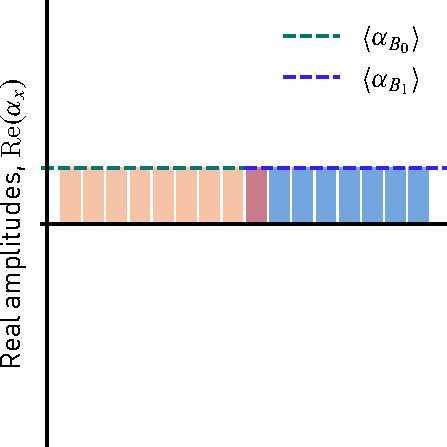
\includegraphics[width=0.33\textwidth]{grover_localiter0}
	}
	\subfloat[\labelFigure{grover_localiter1}]
	{
		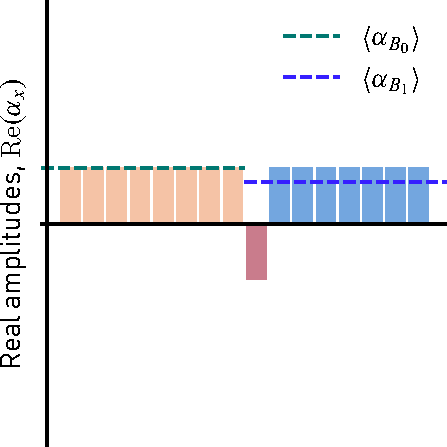
\includegraphics[width=0.33\textwidth]{grover_localiter1}
	}
	\subfloat[\labelFigure{grover_localiter2}]
	{
		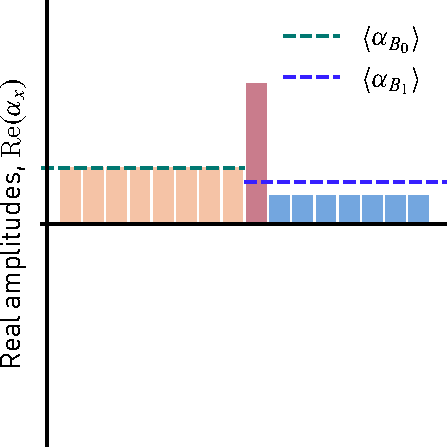
\includegraphics[width=0.33\textwidth]{grover_localiter2}
	}
	\caption[The action of a single local Grover iterate on the level of the amplitudes for a search space of size ${N=2^4}$ and a block size ${b=2^{3}}$, which divides the search into ${K=2}$ blocks.]{The action of a single local Grover iterate on the level of the amplitudes for a search space of size ${N=2^4}$ and a block size ${b=2^{3}}$, which divides the search into ${K=2}$ blocks. $\ev{\alpha_{B_0}}$ and $\ev{\alpha_{B_1}}$ represent the block average for each block. \textbf{(a)} We begin with the uniform superposition state $\ket{\psi}$, the amplitude of target element is indicated in red and the rest of amplitudes in the target block is indicated in blue, while all the amplitudes in the non-target block indicated in orange. \textbf{(b)} After applying the phase oracle the amplitude of the target state acquires a relative minus sign. \textbf{(c)} The action of local diffuser operator $D_{4,3}$ is to invert the amplitudes in each block about the block's average amplitude, thus non-negative amplitudes decrease while negative amplitudes increase in each block; amplifying the amplitude of the target element.}
	\labelFigure{amplitude_localampl}
\end{figure}

\noindent
They further show that the number of iterates (both local and global) for large values of $K$ scales like $~\pi/4\sqrt{N} - c\sqrt{b}$ for a positive constant $c$. Refs.~\cite{Korepin_2005,Korepin_2006,Choi_2006,Korepin_2006a,Korepin_2006b} study various sequence and application orders of $G_{n,m}$ and $G_{n}$ with the aim of reducing the constant $c$, culminating in Ref.~\cite{Korepin_2006} showing that sequences of the kind $G_{n}G_{n,m}^{l_1}G_{n}^{l_2}$ are optimal among different classes of sequences. The values of $l_1,l_2$ can be found by minimizing $S = l_1 + l_2 + 1 \simeq \pi / 4 \sqrt{N} - c \sqrt{b}$ for a certain probability threshold value and number of blocks $K$. Ref.~\cite{Korepin_2005} adopts the parametrization $l_1 = \pi / 4 \sqrt{N} - \eta_K\sqrt{b}$ and $l_2 = \alpha_K\sqrt{b}$ and numerically minimizes $c = (\alpha_K - \eta_K)$; ~\refTableOnly{numeric_vals} shows some values for $\alpha_K$ and $\eta_K$ from the aforementioned reference. The quantum partial search with this sequence of local and global is called the \gls{GRK} algorithm. ~\refEquationOnly{spherical_vec} is suggestive that the partial quantum search algorithm has a similar geometric interpretation as the canonical quantum search. Indeed, $G_{\text{GRK}} = G_{n}G_{n,m}^{l_1}G_{n}^{l_2}$ is an element of the orthogonal group $O(3)$~\cite{Korepin_2006b}.

\begin{figure}[h]
	\subfloat[\labelFigure{grover_order0}]
	{
		% DD DD D
		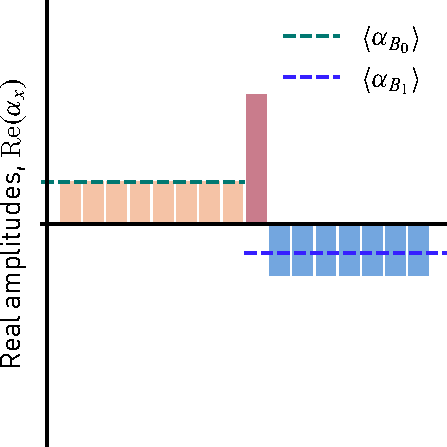
\includegraphics[width=0.33\textwidth]{grover_order0}
	}
	\subfloat[\labelFigure{grover_order1}]
	{
		% DD D DD
		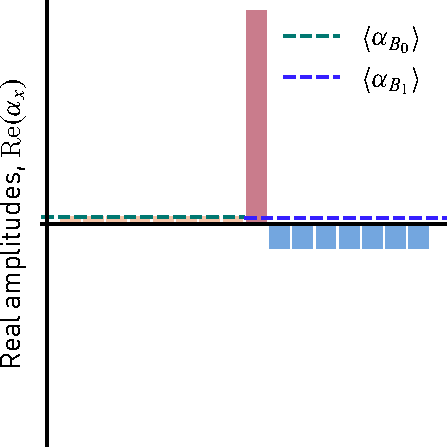
\includegraphics[width=0.33\textwidth]{grover_order1}
	}
	\subfloat[\labelFigure{grover_order2}]
	{
		%% D DD DD
		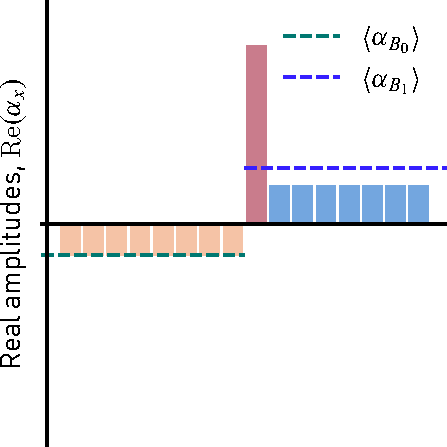
\includegraphics[width=0.33\textwidth]{grover_order2}
	}
	\caption[The actions of different ordering of a global and two local Grover iterates on the level of the amplitudes for ${N=2^4}$, ${b=2^3}$, and ${K=2}$. $\ev{\alpha_{B_0}}$ and $\ev{\alpha_{B_1}}$ represent the block average for each block.]{The actions of different application order of a global and two local Grover iterates on the level of the amplitudes for ${N=2^4}$, ${b=2^3}$, and ${K=2}$. $\ev{\alpha_{B_0}}$ and $\ev{\alpha_{B_1}}$ represent the block average for each block. Action of the application order \textbf{(a)} $G_{4,3}G_{4,3}G_{4}$, \textbf{(b)} $G_{4,3}G_{4}G_{4,3}$, and \textbf{(c)} $G_{4}G_{4,3}G_{4,3}$. The order of operators is important since the local and global Grover operators have non-trivial commutation relations, in all three scenarios we end up with different probabilities for the target element.}
	\labelFigure{iterate_order}
\end{figure}

\bigskip
\noindent
We summarize the \acs{GRK} algorithm to conclude the subsection and show its schematic in~\refFigureOnly{grk_schematic}.

\begin{table}[h]
		\centering
		\caption[Numeric values for $\alpha_K$ and $\eta_K$ for different values of the number of blocks $K$ for the \acs{GRK} algorithm adopted from Korepin et. al]{Numeric values for $\alpha_K$ and $\eta_K$ for different values of the number of blocks $K$ for the \acs{GRK} algorithm, adopted from Ref.~\protect\cite{Korepin_2005}.}
		\labelTable{numeric_vals}
		\begin{tabular}{lll}
			\toprule
			$K$ & $\alpha_K$ & $\eta_K$ \\
			\toprule
			$2$  & $0.7854$     & $1.1107$ \\
			$3$  & $0.65906$    & $0.9961$ \\ 
			$4$  & $0.6155$     & $0.9553$ \\
			$5$  & $0.6155$     & $0.9341$ \\
			$\infty$ & $0.5236$ & $0.866$  \\
			\toprule
		\end{tabular}
\end{table}

\clearpage

\begin{figure}[t!]
	\centering
	\resizebox{1.0\textwidth}{!}{%
	\begin{tikzpicture}
	\begin{yquant}[register/separation=4mm]
		qubit {$\ket{x_{\idx}} = \ket0$} j[2];
		nobit ellipsis;
		qubit {$\ket{x_{m}} = \ket{0}$} jnm;
		nobit ellipsis2;
		qubit {$\ket{x_{n}} = \ket{0}$} jn;
		h j;
		vdots ellipsis;
		h jnm;
		vdots ellipsis2;
		h jn;

		[this subcircuit box style={draw, dashed, inner ysep=6pt, label=above:Repeat $l_1 \simeq \pi / 4 \sqrt{N} - \eta_K\sqrt{b}$ times}]
		subcircuit {
			qubit {} j[2];
			nobit ellipsis;
			qubit {} jnm;
			nobit ellipsis2;
			qubit {} jn;

			[x radius=0.3cm]
			box {$U_{\chi}$} (j-jn);
			h j;
			h jnm;
			h jn;
			[x radius=0.5cm]
			box {$2\op{0}^{\otimes n} - \mathds{1}$} (j-jn);
			h j;
			h jnm;
			h jn;
		} (j, jnm, jn, ellipsis, ellipsis2);

		[this subcircuit box style={draw, dashed, inner ysep=6pt, label=above:Repeat $l_2 \simeq \alpha_K\sqrt{b}$ times}]
		subcircuit {
			qubit {} j[2];
			nobit ellipsis;
			qubit {} jnm;
			nobit ellipsis2;
			qubit {} jn;

			[x radius=0.3cm]
			box {$U_{\chi}$} (j-jn);
			h j;
			h jnm;
			[x radius=0.5cm]
			box {$2\op{0}^{\otimes m} - \mathds{1}_{2^m}$} (j-jnm);
			h j;
			h jnm;
		} (j, jnm, jn, ellipsis, ellipsis2);

		[x radius=0.3cm]
		box {$U_{\chi}$} (j-jn);
		h j;
		h jnm;
		h jn;
		[x radius=0.5cm]
		box {$2\op{0}^{\otimes n} - \mathds{1}$} (j-jn);
		h j;
		h jnm;
		h jn;


		measure j;
		vdots ellipsis;
		measure jnm,jn;
	\end{yquant}
	\end{tikzpicture}
	}
	\caption[A schematic circuit diagram of the \acs{GRK} algorithm.]{A schematic circuit diagram of the \acs{GRK} algorithm; which begins with all $n$ qubits in the state $\ket{0}$, after which a Hadamard gate $H$ is applied to all qubits to create a uniform superposition of $2^n$ basis states. A sequence of $l_1$ global Grover operators, followed by a sequence of $l_2$ local Grover iterates, and lastly a single global Grover operator is applied to the uniform superposition. Measuring in the computational basis, the target element will be found with high probability.}
	\labelFigure{grk_schematic}
\end{figure}


\bigskip
\begin{enumerate}
\item \emph{Initialization}\newline
Prepare $\ket{0}^{\otimes n}$ and apply $H^{\otimes n}$ on all the qubits, creating a uniform superposition of $N=2^n$ basis states:
\begin{align*}
    \ket{0}^{\otimes n} \to \frac{1}{\sqrt{N}}\displaystyle\sum_{x=0}^{N-1} \ket{x}
\end{align*}

\item \emph{Global Grover iterates}\newline
Apply the global Grover iterates $l_1 \simeq \pi / 4 \sqrt{N} - \eta_K\sqrt{b}$ times:
\begin{align*}
	\frac{1}{\sqrt{N}}\displaystyle\sum_{x=0}^{N-1} \ket{x} \to \frac{1}{\sqrt{N}}\displaystyle\sum_{x=0}^{N-1} G_{n}^{l_1}\ket{x}
\end{align*}

\item \emph{Local Grover iterates}\newline
Apply local Grover iterates $l_2 \simeq \alpha_K\sqrt{b}$ times: 

\begin{align*}
	\frac{1}{\sqrt{N}}\displaystyle\sum_{x=0}^{N-1} G_{n}^{l_1}\ket{x} \to \frac{1}{\sqrt{N}}\displaystyle\sum_{x=0}^{N-1} G_{n,m}^{l_2}G_{n}^{l_1}\ket{x}
\end{align*}

\item \emph{Single global Grover iterate}\newline
Apply a single global Grover iterate: 

\begin{align*}
	\frac{1}{\sqrt{N}}\displaystyle\sum_{x=0}^{N-1} G_{n,m}^{l_2}G_{n}^{l_1}\ket{x} \to \frac{1}{\sqrt{N}}\displaystyle\sum_{x=0}^{N-1} G_{n} G_{n,m}^{l_2}G_{n}^{l_1}\ket{x}
\end{align*}


\item \emph{Measurements}\newline
    Measure all qubits in the computational basis yielding a target element with high probability. In case of failure, go back to step 1.
\end{enumerate}

\section{Survey of recent results relating to NISQ processors}
\labelSection{C2_survey_of_recent_results_on_nisq_processors}
As we have seen in sections ~\refSectionOnly{C2_canonical_construction_of_grovers_algorithm} and ~\refSectionOnly{C2_partial_search_quantum_algorithm}, both the canonical and partial quantum search algorithms in various scenarios have been proven to be optimal in the number of steps they undertake to solve the search problem. However, as I briefly alluded to in the opening of this chapter, in physical implementations (emphasis on \acs{NISQ} processors) of any quantum algorithm, each of these steps are broken down into intermediary subroutines and further into physically realizable atomic operations in the universal gate set of a particular physical implementation. 

\bigskip
\noindent
For physical realizations of quantum search algorithms, the Grover iterates constitute the most resource intensive parts of the algorithm in terms of such atomic operations. The phase oracle $U_{\chi}$ in the Grover iterate is equivalent to an $n$-qubit controlled-$Z$ gate (modulo single qubit gates). Suppose our unique target element is the computational basis state $\ket{b_0b_1b_2\cdots b_{n-1}}$, then following circuit composed of Pauli $X$ gate and $n$-qubit controlled-$Z$, $C^{n-1}[Z]$ gates, implements a phase oracle $U_{\chi}$ that gives the state $\ket{b_0b_1b_2 \cdots b_{n-1}}$ a relative negative amplitude~\footnote[][-50pt]{For $n=2$, it is equivalent to a controlled-$Z$ and for $n=3$ it is equivalent to a controlled-controlled-$Z$ gate.}.

\begin{figure}[h]
    \centering
	\begin{tikzpicture}
		\begin{yquant}[register/separation=2mm]
			qubit {$b_{\idx}$} q[2];
			[name=wave, register/minimum height=8mm]
			nobit wave;
			qubit {$b_{n-2}$} qm;
			qubit {$b_{n-1}$} qn;
			box {$X^{\neg b_0}$} q[0];
			box {$X^{\neg b_1}$} q[1];
			vdots wave;
			box {$X^{\neg b_{n-2}}$} qm;
			box {$X^{\neg b_{n-1}}$} qn;
			box {$Z$} qn | q[0],q[1], qm;
			box {$X^{\neg b_0}$} q[0];
			box {$X^{\neg b_1}$} q[1];
			vdots wave;
			box {$X^{\neg b_{n-2}}$} qm;
			box {$X^{\neg b_{n-1}}$} qn;
		\end{yquant}
	\end{tikzpicture}
    \caption[A circuit diagram that realizes a general phase oracle in Grover's algorithm.]{A circuit diagram that realizes a general phase oracle in Grover's algorithm; the circuit maps ${\ket{b_0b_1b_2 \cdots b_{n-1}} \to -\ket{b_0b_1b_2 \cdots b_{n-1}}}$, where $(X_a)^{b_a}$ applies a Pauli $X$ gate to qubit a if $b_a=1$ and applies the identity if $b_0$. $Z$ denotes the Pauli $Z$ gate}
	\labelFigure{phase_oracle_circ}
\end{figure}

\noindent
where $\neg 0 = 1$ and $\neg 1 = 0$.  The diffuser operator $G_n$ is implemented similarly

\begin{figure}[h]
    \centering
	\begin{tikzpicture}
		\begin{yquant}[register/separation=2mm]
			qubit {$b_{\idx}$} q[2];
			[name=wave, register/minimum height=8mm]
			nobit wave;
			qubit {$b_{n-2}$} qm;
			qubit {$b_{n-1}$} qn;
			h q;
			box {$X$} q[0];
			box {$X$} q[1];
			vdots wave;
			h qm;
			h qn;
			box {$X$} qm;
			box {$X$} qn;
			box {$Z$} qn | q[0],q[1], qm;
			box {$X$} q[0];
			box {$X$} q[1];
			h q;
			vdots wave;
			box {$X$} qm;
			box {$X$} qn;
			h qm;
			h qn;
		\end{yquant}
	\end{tikzpicture}
    \caption[A circuit diagram that realizes a global diffuser operator in Grover's algorithm.]{A circuit diagram that realizes a global diffuser operator in Grover's algorithm, where $X, Z, H$ are the Pauli $X,Z$ and $H$ is the Hadamard gate respectively.}
	\labelFigure{diffuser_circ}
\end{figure}

\noindent
 As we have seen, these two operators (the Grover iterate $D_{n}U_{\chi}$) must be repeated several times to guarantee some threshold for the probability of success. For \acs{NISQ} processors, the $n$-qubit controlled-$Z$ gate for more than two qubits is not an atomic operation. The $n$-qubit controlled-$Z$ gate is equivalent to a generalized $n$-qubit Toffoli gate, $C^{n-1}[X]$, by applying a Hadamard gate $H$ to the target qubit just before and after the gate (\ie $HZH = X$). The generalized $n$-qubit Toffoli gate itself is also not an atomic operation on \acs{NISQ} processors, but instead decomposed into atomic operations (controlled-NOT and single qubits). The two-qubit gate such as the controlled-NOT gate are physically realized through two-qubit interactions that induce conditional dependence of the state of one qubit to the other, for instance a cross-resonance interaction for superconducting qubits~\cite{Kjaergaard_2020} and Mølmer-Sørensen interaction for trapped ions qubits~\cite{Bruzewicz_2019}. The commonality across \acs{NISQ} architectures is that such two-qubit interactions are non-trivial, making them experimentally expensive and much more prone to errors than single-qubit gates. Hence, for reasons motivated by practicality, the analysis of circuit complexity is done usually in terms of the two-qubit gate count in a circuit.

 \bigskip
 \noindent
 For $n=3$, the controlled-controlled-$Z$ (hence the controlled-controlled-NOT gate) gate cannot be implemented with less than five two-qubit gates~\cite{Yu_2013}; the traditional three-qubit decomposition shown in~\refFigureOnly{control_control_z}, uses six controlled-NOT and seven $T/T^{\dagger}$ gates, has shown to be optimal in terms of controlled-NOT count~\cite{Shende_2008}. However, for $n\geq4$ the exact controlled-NOT count of its decomposition without the use auxiliary of qubits is not known~\cite{Shende_2008}. He~\etal~\cite{He_2017} have shown that if a single auxiliary qubit is provided $24n − 72$ controlled-NOT gates suffice.

\clearpage
\begin{figure}[t!]
	\centering
	\begin{tikzpicture}
		\begin{yquantgroup}[register/separation=2mm]
			\registers{
				qubit {} q[3];
			}
			\circuit{
				box {$Z$} q[2] | q[0-1];
			}

			\equals 

			\circuit{
				cnot q[2] | q[1];
				box {$T^\dagger$} q[2];
				cnot q[2] | q[0];
				box {$T$} q[2];
				cnot q[2] | q[1];
				box {$T^\dagger$} q[2];
				cnot q[2] | q[0];
				box {$T$} q[2];
				box {$T$} q[1];
				cnot q[1] | q[0];
				box {$T^\dagger$} q[1];
				box {$T$} q[0];
				cnot q[1] | q[0];
			}


		\end{yquantgroup}
	\end{tikzpicture}
	\caption[A circuit diagram showing the decomposition of a controlled-controlled-$Z$ gate in terms of elementary gates.]{A circuit diagram showing the decomposition of a controlled-controlled-$Z$ gate in terms of elementary gates; six controlled-NOT and seven $T/T^{\dagger}$ gates.}
	\labelFigure{control_control_z}
\end{figure}

\noindent
Additionally, they show that if $n-1$ auxiliary qubits are provided, then $4n − 7$ controlled-NOT gates suffice. With such a decomposition it is possible to trade for a great reduction of controlled-NOT gates at the expensive of using more qubits. The unavoidable consequence for physical implementations is that, it becomes much harder to maintain quantum coherence as the relevant Hilbert space is much larger (from $2^n$ to $2^{2n -1}$ possible states). Furthermore, \acs{NISQ} processors have limited connectivity among the qubits on the physical device hence multi-qubit gates cannot be performed directly on qubits that are not directly connected, and instead must be done by way of appropriate SWAP gates; a single SWAP gate costs three controlled-NOT gates, as shown in~\refFigureOnly{swap_gate}

\begin{figure}[h]
    \centering
	\begin{tikzpicture}
		\begin{yquantgroup}[register/separation=8mm]
			\registers{
				qubit {} q[2];
			}

			\circuit{
				swap (q[0, 1]);
			}

			\equals

			\circuit{
				cnot q[1] | q[0];
				cnot q[0] | q[1];
				cnot q[1] | q[0];
			} 
		\end{yquantgroup}
	\end{tikzpicture}
    \caption[A circuit diagram showing the decomposition of a SWAP gate in terms of elementary gates.]{A circuit diagram showing the decomposition of a SWAP gate in terms of elementary gates; three controlled-NOT gates.} 
	\labelFigure{swap_gate}
\end{figure}

\noindent
The theoretical reduction of the controlled-NOT gate count gained by the use of auxiliary qubits in practice may be lost depending on the connectivity of the physical device. Besides, the two-qubit gate count, another way circuit complexity is examined is in terms of its circuit depth. Circuit depth is the number of consecutive parallel operations in a circuit from its input to output. Each such parallel operation can be counted as a single step, and thus circuit depth can be taken to be a good proxy for algorithmic time. Analysis in terms of circuit depth is also motivated by practicality, since \acs{NISQ} processors have short-lived coherence times, over which a computation can remain fully coherent, and thus limited to realizing shallow depth circuits~\cite{Preskill_2018}. The aforementioned decomposition of an $n$-qubit Toffoli due to He~\etal~\cite{He_2017} has a linear depth $\bigO{n}$ and logarithmic depth $\bigO{\log{n}}$ for a single auxiliary qubit and $n-1$ auxiliary qubits, respectively.

\subsection{Depth optimization of the quantum search}
\labelSection{C2_depth_optimization_of_the_quantum_search}
On the account of the limitations of \acs{NISQ} processors,~\ie the short-lived coherence time, limited number of qubits and limited connectivity among qubits, an analysis by Zhang and Korepin~\cite{Zhang_2020} emphasizes the imperative of designing algorithms in such a way that is aware of these limitations. Inspired by the \acs{GRK} algorithm, and these practical considerations, they proposed a modification of the quantum search algorithm that is optimal in circuit depth, not necessarily optimal in the number of steps with respect to achieving some probability threshold. To facilitate this optimization, they define a figure of merit $\alpha$, that is a ratio of the depth of the phase oracle depth and depth of the diffuser operator $D_n$

\begin{align}
	\labelEquation{depth_ratio}
	\alpha = \frac{d(U_{\chi})}{d(D_n)},
\end{align}

\noindent
for single-target oracle implementations of the kind in~\refFigureOnly{phase_oracle_circ} and global diffuser operator of the kind in~\refFigureOnly{diffuser_circ}, since the dominating circuit depth arises from the $n$-qubit controlled-$Z$ gate, it is expected that $\alpha=1$. 

\clearpage
\noindent
Recall that the local diffuser operators $D_{n,m}$ act on a small subspace  $m < n$, thus in theory require fewer elementary operators and have lower depth than the global diffuser operators, at the cost of reducing the success probability\footnote{This is clear from the perspective of~\refFigureOnly{diffuser_circ}, we expect an $m$-qubit controlled-$Z$ gate will decomposed into fewer elementary gates than $n$-qubit controlled-$Z$ gate if $m < n$.}; hence their optimization method is based on the replacement of global diffuser operators with local diffuser operators to minimize the depth of Grover's algorithm, while taking into account the trade-off in the probability of success. Similar to the \acs{GRK} algorithm, they consider a general sequence of local ($G_m$) and global Grover iterate operators ($G_n$) of the form

\begin{align}
	\labelEquation{local_optimal_seq}
	S_{n,m}(\bar{l}) =  G_n^{l_1} G_m^{l_2} \cdots G_n^{l_{q-1}}G_m^{l_q},
\end{align}

\noindent
here $\bar{l} = (l_1, l_2, \ldots, l_q)$ is a tuple of natural numbers, $l_\text{tot} = \sum_{p=1}^{q}l_p$ is the total number of Grover iterates (both local and global). For instance, $S_{n}(l,0)=G_n^l$ is the canonical Grover algorithm. The notational convention is that last number $l_q$ is always the number of local Grover iterate operators, thus in this notation the Grover iterate for the \acs{GRK} is denoted by $S_{n,m}(1,l_2,l_1,0) = G_n^{1}G_m^{l_2}G_n^{l_1}G_m^{0}$. Furthermore, the above notation only considers local Grover iterate operators acting on the same qubit subspace with the same block size $m$. For such a sequence of Grover iterates, the probability of measuring the target element $\ket{s}$ is given by

\begin{align}
	P_{n,m}(\bar{l}) = \abs{\mel{s}{S_{n,m}(\bar{l})H^{\otimes n}}{0}^{\otimes n}}^2.
\end{align}

\noindent
From this, they define the ratio of the expected depth for the Grover iterate sequence $S_{n,m}$ and its probability of success as 

\begin{align}
	\tilde{d}(\alpha) = \frac{d(S_{n,m}(\bar{l}))}{P_{n,m}(\bar{l})},
\end{align}

\noindent
and minimize the above quantity with respect both $m \geq 2$ and the tuple of natural numbers $\bar{l}$.

\begin{align}
	\tilde{d}(\alpha) = \underset{m, \bar{l}}{\text{minimize }}\frac{d(S_{n,m}(\bar{l}))}{P_{n,m}(\bar{l})}.
\end{align}

\noindent
The study in Ref.~\cite{Zhang_2020} report that below certain threshold values of $\alpha$ for $n\geq4$, their algorithm gives rise to sequences that have lower expected depth than the canonical algorithm, that is, the canonical algorithm is not optimal in depth\footnote[][-25pt]{${S_{n}(l,0) = G_n^l}$, for ${l = \left\lfloor 0.583 \sqrt{N} \right\rfloor}$. Recall from~\refSectionOnly{C2_depth_optimization_of_the_quantum_search} this value of $l$ gives the least expected number of iterations, and thus the minimal expected depth, for a ${P_{n}(l) \simeq 0.845}$ probability of success.}. Ref.~\cite{Zhang_2020} gives examples of depth-optimal sequences $S_{n,m}(\bar{l})$ for $\alpha=1$, $n \in {3,4,\ldots, 10}$, in comparison with the canonical sequence with only global Grover iterates $S_{n}$; shown in~\refTableOnly{global_optimal_seq} and~\refTableOnly{local_optimal_seq}, respectively.

\begin{table}[h!]
	\centering
	\caption[The minimum expected depth for the quantum search algorithm for the sequence of the kind ${S_{n}(l,0) = G_n^{l}}$.]{The minimum expected depth for the quantum search algorithm for the sequence of the kind ${S_{n}(l,0) = G_n^{l}}$, where ${l = \left\lfloor 0.583 \sqrt{N} \right\rfloor}$ from~\protect\refEquationOnly{local_optimal_seq}, where the ratio in~\protect\refEquationOnly{depth_ratio} is set to ${\alpha=1}$; adopted from Ref.~\cite{Zhang_2020}.}
	\labelTable{global_optimal_seq}
	\begin{tabular}{ccccc}
		\toprule
		$n$ & $S_n(\bar{l})$ & $P_{n}(\bar{l})$ & $d\left(S_n(\bar{l})\right)$ & $\tilde{d}(\alpha = 1)$\\
		\toprule
		$4$  & $S_4(1,0)$     & $0.473$ & $30$   & $64.47$    \\
		$5$  & $S_5(2,0)$     & $0.602$ & $124$  & $205.83$   \\ 
		$6$  & $S_6(4,0)$     & $0.816$ & $504$  & $617.36$   \\
		$7$  & $S_7(6,0)$     & $0.833$ & $1446$ & $1756.35$  \\
		$8$  & $S_8(9,0)$     & $0.861$ & $2916$ & $3388.03$  \\
		$9$  & $S_9(12,0)$    & $0.798$ & $4848$ & $6071.76$  \\
		$10$ & $S_{10}(18,0)$ & $0.838$ & $8712$ & $10397.28$ \\
		\toprule
	\end{tabular}
\end{table}

\bigskip
\bigskip

\begin{table}[h!]
	\centering
	\caption[The minimum expected depth for the quantum search algorithm for the sequence of the kind ${S_{n,m}(\bar{l}) = G_n^{l_1} G_m^{l_2} \cdots G_n^{l_{q-1}}G_m^{l_q}}$.]{The minimum expected depth for the quantum search algorithm for the sequence of the kind ${S_{n,m}(\bar{l}) = G_n^{l_1} G_m^{l_2} \cdots G_n^{l_{q-1}}G_m^{l_q}}$ from~\protect\refEquationOnly{local_optimal_seq}, where the ratio in~\protect\refEquationOnly{depth_ratio} is set to ${\alpha=1}$; adopted from Ref.~\cite{Zhang_2020}.}
	\labelTable{local_optimal_seq}
	\begin{tabular}{ccccc}
		\toprule
		$n$ & $S_{n,m}(\bar{l})$ & $P_{n,m}(\bar{l})$ & $d\left(S_{n,m}(\bar{l})\right)$ & $\tilde{d}(\alpha = 1)$\\
		\toprule
		$4$  & $S_{4,3}(1,1)$     				 & $0.821$ & $52$   & $63.32$    \\
		$5$  & $S_{5,4}(1,1,1)$     			 & $0.849$ & $154$  & $181.48$   \\ 
		$6$  & $S_{6,4}(1,1,2)$     			 & $0.755$ & $360$  & $475.97$   \\
		$7$  & $S_{7,4}(1,1,2,1,2)$     		 & $0.887$ & $1173$ & $1322.75$  \\
		$8$  & $S_{8,4}(1,1,2,1,2,1,2)$          & $0.875$ & $2211$ & $2527.43$  \\
		$9$  & $S_{9,5}(1,1,2,1,2,1,2,1,2)$      & $0.831$ & $3713$ & $4470.20$  \\
		$10$ & $S_{10,5}(1,1,2,1,2,1,2,1,2,1,2)$ & $0.847$ & $6453$ & $7614.56$ \\
		\toprule
	\end{tabular}
\end{table}

\bigskip
\bigskip

\subsection{Multi-stage strategy for quantum search}
\labelSection{C2_multi_stage_for_quantum_search}
Another significant contribution from Ref.~\cite{Zhang_2020} is a multi-stage quantum search algorithm that divides the quantum search algorithm into separate circuits (with reinitializations and measurements) that each find the $m$ bits of the target element $\ket{s}$ (similar to the partial search). Each subsequent stage is dependent on the results of the preceding stage to reinitialize the subsequent circuit such that the first $m_1$ bits of the target are those found from the preceding, then find another $m_2$ of the target element. This process is repeated until we have all the bits of the target element are recovered. In each subsequent stage, the diffuser operators no longer act on the reinitialized subspace from the preceding stage. This greatly reduces the number of elementary operations (hence circuit depth) in each subsequent stage. The great advantage of such a multi-stage algorithm is mostly due to the reinitializations, since coherence no longer has tp be maintained over one long circuit, and is renewed on each reinitialization, preventing the effects of noise from accumulating. The steps for a two-stage quantum search from Ref.~\cite{Zhang_2020} are given below and the circuit diagram schematic is shown in~\refFigureOnly{multi_stage_schematic}

\begin{enumerate}
\item \emph{Initialization}\newline
Prepare $\ket{0}^{\otimes n}$ and apply $H^{\otimes n}$ on all the qubits, creating a uniform superposition of $N=2^n$ basis states:
\begin{align*}
    \ket{0}^{\otimes n} \to \frac{1}{\sqrt{N}}\displaystyle\sum_{x=0}^{N-1} \ket{x}.
\end{align*}

\noindent
The target element is $\ket{s}$ is bipartitioned into $\ket{s} = \ket{s_1}\otimes\ket{s_2}$, where $s_1$ is $m_1$ bits long and $s_2$ is $m_2$ bits long such that $m_1 + m_2 = n$.

\item \emph{Finding }$\ket{s_1}$\newline
Apply the sequence of Grover iterates $S_{n,m_2}(\bar{l}) = G_n^{l_1} G_{m_2}^{l_2} \cdots G_n^{l_{q-1}}G_{m_2}^{l_q}$:

\begin{align*}
	\frac{1}{\sqrt{N}}\displaystyle\sum_{x=0}^{N-1} \ket{x} \to \frac{1}{\sqrt{N}}\displaystyle\sum_{x=0}^{N-1} S_{n,m_2}(\bar{l})\ket{x},
\end{align*}

\noindent
where the local Grover operator $G_{m_2}$ are acting on the  $m_2$ qubit subspace.

\item \emph{First round of measurements}\newline
    Measure the on the $m_1$ qubit subspace in the computational basis; Suppose we obtain the bit string outcome $b = b_0b_1\cdots b_{m_1-1}$; the probability for obtaining this outcome is denoted by $P_{n, m_2}^{(1)}(\bar{l})$.


\item \emph{Reinitialization}\newline
Restart the computation to $\ket{0}^{\otimes n}$ and prepare the state $\ket{b_0b_1\cdots b_{m_1}}$ on the first $m_1$ qubits by applying $X^{b_0}\otimes X^{b_1}\otimes\cdots\otimes X^{b_m}$ on $\ket{0}^{\otimes n}$.  Apply $H^{\otimes m_2}$ on the $m_2$ qubit subspace, creating a uniform superposition of $M=2^{m_2}$ basis states on this subspace:

\begin{align*}
    X^{b_0}\otimes X^{b_1}\otimes\cdots\otimes X^{b_m} H^{\otimes m_2} \ket{0}^{\otimes n} \to \frac{1}{\sqrt{M}}\displaystyle\sum_{x=0}^{M-1} \ket{b_0b_1\cdots b_{m_1-1}}\otimes\ket{x}.
\end{align*}

\item \emph{Finding $\ket{s_2}$}\newline
Apply the sequence of Grover iterates $S_{m_2,m'}(\bar{l'}) = G_{m_2}^{l'_1} G_{m_2,m'}^{l'_2} \cdots G_{m_2}^{l'_{q-1}}G_{m_2, m'}^{l'_q}$:

\begin{align*}
	\frac{1}{\sqrt{M}}\displaystyle\sum_{x=0}^{M-1} \ket{b_0b_1\cdots b_{m_1 -1}}\otimes\ket{x} \to \frac{1}{\sqrt{M}}\displaystyle\sum_{x=0}^{M-1} \ket{b_0b_1\cdots b_{m_1 - 1}}\otimes S_{m_2,m'}(\bar{l'})\ket{x}.
\end{align*}

\item \emph{Second round of measurements}\newline
    Measure the on the $m_2$ qubit subspace in the computational basis; Suppose we obtain the bit string outcome $b' = b'_0b'_1\cdots b'_{m_2-1}$, the probability for obtaining this outcome is denoted by $P_{m_2, m'}^{(2)}(\bar{l'})$.

\item \emph{Verify solution} \newline
	We verify the solution $s = b_1b_2\cdots b_{m_1-1} b'_{m_1}b'_{m_1+1}\cdots b'_{n}$ by simply checking the boolean function $\chi$ in~\refEquationOnly{check_function} if $\chi(s) = 1$. If it happens that $\chi(s) = 0$, then we go back to step 1.

\end{enumerate}

\begin{figure}[t!]
	\centering
	\subfloat[]{
	\resizebox{1.0\textwidth}{!}{%
	\begin{tikzpicture}
	\begin{yquant}[register/separation=4mm]
		qubit {$\ket{x_{\idx}} = \ket0$} j[2];
		nobit ellipsis;
		qubit {$\ket{x_{m_1-1}} = \ket{0}$} jnm;
		nobit ellipsis2;
		qubit {$\ket{x_{n}} = \ket{0}$} jn;
		h j;
		vdots ellipsis;
		h jnm;
		vdots ellipsis2;
		h jn;

		[x radius=0.5cm]
		box {$U_{\chi}$} (j-jn);

		[x radius=0.5cm]
		box {$D_{m_1}$} (j-jnm);

		[draw=none]
		box {$\dots$} j-jn;

		[x radius=0.5cm]
		box {$U_{\chi}$} (j-jn);

		[x radius=0.5cm]
		box {$D_{n}$} (j-jn);

		[draw=none]
		box {$\dots$} j-jn;

		[x radius=0.5cm]
		box {$U_{\chi}$} (j-jn);
		[x radius=0.5cm]
		box {$D_{m_1}$} (j-jnm);

		vdots ellipsis;
		measure j,jnm;

		output {$b_{\idx}$} j;
		output {$b_{m_1-1}$} jnm;
	\end{yquant}
	\end{tikzpicture}
	}
	} \\
	\subfloat[]
	{
	\resizebox{1\textwidth}{!}{%
	\begin{tikzpicture}
	\begin{yquant}[register/separation=4mm]
		qubit {$\ket{x_{\idx}} = \ket0$} j0;
		nobit ellipsis;
		qubit {$\ket{x_{m_1-1}} = \ket{0}$} jm1;
		qubit {$\ket{x_{m_2}} = \ket{0}$} jm2;
		nobit ellipsis2;
		qubit {$\ket{x_{m_2+m'}} = \ket{0}$} jm3;
		nobit ellipsis3;
		qubit {$\ket{x_{n}} = \ket{0}$} jn;

		box {$X^{b_0}$} j0;
		vdots ellipsis;
		box {$X^{b_{m_1 - 1}}$} jm1;

		h jm2;
		vdots ellipsis2;
		h jm3;
		vdots ellipsis3;
		h jn;

		[x radius=0.5cm]
		box {$U_{\chi}$} (j0-jn);
		[x radius=0.5cm]
		box {$D_{m'}$} (jm2-jm3);
	

		[draw=none]
		box {$\dots$} j0-jn;


		[x radius=0.5cm]
		box {$U_{\chi}$} (j0-jn);

		[x radius=0.5cm]
		box {$D_{m_2}$} (jm2-jn);

		[draw=none]
		box {$\dots$} j0-jn;

		[x radius=0.5cm]
		box {$U_{\chi}$} (j0-jn);

		[x radius=0.5cm]
		box {$D_{m'}$} (jm2-jm3);

		measure jm2;
		vdots ellipsis2;
		measure jm3;
		hspace {1.10cm} ellipsis3;
		vdots ellipsis3;
		hspace {1.10cm} jn;
		measure jn;

		output {$b_{m_2}$} jm2;
		output {$b_{m_2+m'}$} jm3;
		output {$b_{n}$} jn;

	\end{yquant}
	\end{tikzpicture}
	}
	}
	\caption[A schematic circuit diagrams for the two-stage quantum search algorithm.]{A schematic circuit diagrams for the two-stage quantum search algorithm; \textbf{(a)} In the first stage a sequence of local and global diffuser operators are used in conjunction to search for the first $m_1$ bits of the target element, where the local diffuser operators act on the first subspace of $m_1$ qubits, at the end of this stage, these qubits are measured in computational basis. \textbf{(b)} The second stage begins by first preparing the measured outcome from the first stage in the first $m_1$. Then a sequence of local diffuser operators are applied on the $m_2$ qubit space and on a smaller subspace of $m'$ qubits. At end of this stage we measure all $m_2$ in the computational basis to recover the last $m_2$ bits of the target element.} 
	\labelFigure{multi_stage_schematic}
\end{figure}


\noindent
Similarly, as they define the expected depth for the two-stage algorithm for the different sequences in the algorithm
\begin{align}
	\tilde{d}(\alpha) = \frac{d(S^{(1)}_{n,m_2}(\bar{l})) + S^{(2)}_{m_2,m'}(\bar{l'}))}{P_{n,m_2}^{(1)}(\bar{l})P_{m2, m'}^{(2)}(\bar{l'})},
\end{align}

\noindent
and minimize the above quantity with respect to $m_2, m'$ and $\bar{l},\bar{l'}$

\begin{align}
	\tilde{d}(\alpha) = \underset{m_2,m',\bar{l},\bar{l'}}{\text{minimize }}\frac{d(S^{(1)}_{n,m_2}(\bar{l})) + S^{(2)}_{m_2,m'}(\bar{l'}))}{P_{n,m_2}^{(1)}(\bar{l})P_{m2, m'}^{(2)}(\bar{l'})}.
\end{align}

\noindent
The optimal two-stage quantum search sequences for $\alpha=1$, $n \in \{3,4,\ldots, 10\}$ are shown in~\refTableOnly{two_stage_optimal_seq}. 


\begin{table}[h]
	\centering
	\caption[The minimum expected depth for the two-stage quantum search algorithm  where the ratio in~\protect\refEquationOnly{depth_ratio} is set to ${\alpha=1}$.]{The minimum expected depth for the two-stage quantum search algorithm where the ratio in~\protect\refEquationOnly{depth_ratio} is set to ${\alpha=1}$; adopted from Ref.~\cite{Zhang_2020}.}
	\labelTable{two_stage_optimal_seq}
	\resizebox{1.0\textwidth}{!}{%
	\begin{tabular}{cccccccc}
		\toprule
		& \multicolumn{2}{c}{$S_{n,m}(\bar{l})$} & \multicolumn{2}{c}{$P_{n,m}(\bar{l})$} & \multicolumn{2}{c}{$d(S_{n,m}(\bar{l}))$} & \\
		\cmidrule(lr){2-3}\cmidrule(lr){4-5}\cmidrule(lr){6-7}
		$n$ & Stage 1 & Stage 2 & Stage 1 & Stage 2 & Stage 1 & Stage 2 & $d(\alpha=1)$ \\
		\toprule
		$4$  &  $S_{4,2}(1,1)$         & $S_{2,0}(1,0)$   & $0.953$ & $1$     & $48$   & $18$   & $69.25$   \\
		$5$  &  $S_{5,2}(1,1)$         & $S_{2,0}(1,0)$   & $0.658$ & $1$     & $96$   & $34$   & $197.51$  \\
		$6$  &  $S_{6,2}(1,1,1,1)$     & $S_{2,0}(1,0)$   & $0.791$ & $1$     & $384$  & $66$   & $569.22$  \\
		$7$  &  $S_{7,4}(1,4)$         & $S_{2,0}(2,0)$   & $0.739$ & $0.908$ & $792$  & $274$  & $1587.09$ \\
		$8$  &  $S_{8,5}(1,4,1,2)$     & $S_{5,4}(1,1,2)$ & $0.882$ & $0.998$ & $1806$ & $724$  & $2876.40$ \\
		$9$  &  $S_{9,5}(1,4,1,3,1,3)$ & $S_{5,4}(1,1,2)$ & $0.096$ & $0.998$ & $3542$ & $884$  & $4898.88$ \\
		$10$ &  $S_{10,5}(1,4,1,3,1,3,1,3)$ & $S_{5,4}(1,1,2)$ & $0.810$ & $0.998$ & $5485$ & $1044$ & $8081.89$ \\
		\toprule
	\end{tabular}
	}
\end{table}


\bigskip
\noindent
The multi-stage quantum search algorithm also lends itself to a natural way to parallelization, that is, having each stage run on a different quantum processor~\cite{Zhang_2020}. However, unlike a parallelized classical unstructured search, it is not clear that such a parallelization would offer significant improvements in performance (in terms of number of steps) over the multi-stage quantum search algorithm on a single processor; for the canonical algorithm, the performance of such parallelization and multi-stage quantum search (not necessarily depth-optimal) are asymptotically equivalent~\cite{Zalka_1999}.

\bigskip
\subsection{Implementations on NISQ processors}%
\labelSection{C2_implementations_on_nisq_processors}
The first (of great value) of the results of implementations of quantum search algorithms on \acs{NISQ} processors is due to Wang and Kristic~\cite{Wang_2020}, who provided a thorough analysis of the performance of the quantum search algorithms presented here under different sources of errors and decoherence afflicting \acs{NISQ} processors. By way of simulation, they consider the effects of gate errors such as phase, bit flips and depolarizing noise, and dissipative decoherence mechanisms such as amplitude and phase damping, with an increasing number of qubits used. To facilitate their analysis, they define a metric $S$ they call selectivity 

\begin{align}
	S = 10 \log_{10}{(P_{s} / P_{hn})},
\end{align}

\noindent
that quantifies the signal-to-noise of the measured probability of the target element (signal) $P_{s}$, in comparison to the highest measured probability among the non-target states (noise) $P_{hn}$. A negative value for the selectivity is deemed to indicate the search was unsuccessful as the measured probability of the target state is indistinguishable from the noise, \ie $P_{hn} > P_{s}$. 

\clearpage
\noindent
In this way, the analysis is of how much of the various sources of noise can afflict a quantum search algorithm before the selectivity goes below a certain threshold, above which they consider the search to be successful, and defines the greatest strength of the afflicting noise source tolerated by the algorithm~\cite{Wang_2020}.

\bigskip
\noindent
The results in the aforementioned reference show that the depth-optimized quantum search algorithm of Ref.~\cite{Zhang_2020}, particularly the two-stage variant has better tolerance than the canonical algorithm under the various noise sources. Additionally, if one incorporates the use of $n$-qubit controlled-NOT gates that use one auxiliary qubit of the form in Ref.~\cite{Barenco_1995}, the noise resilience of both the canonical and depth-optimized quantum search algorithms can be improved. This improvement is cited as due to the reduction in the number of elementary gates in comparison to using $n$-qubit controlled-NOT gates without auxiliary qubits\footnote{The $n$-qubit controlled-NOT gate synthesis due to Barenco~\etal~\cite{Barenco_1995} uses $48n-208$ controlled-NOT gates with a linear depth; a much more economical synthesis is due to He~\etal~\cite{He_2017}, which uses $24n - 72$.}.


\bigskip
\noindent
The first experimental demonstration to this topic of research of a four-qubit quantum search algorithm on a real \acs{NISQ} processor is due to Gwinner~\etal~\cite{Gwinner_2020}. Distinct from the schemes presented here thus far, both constructions of the phase oracle and diffuser operators in Ref.~\cite{Gwinner_2020} are tailored towards the connectivity of the \acs{NISQ} processors. Their circuit for the four-qubit case of Grover's algorithm uses local diffuser operators with controlled-controlled-$Z$ gates aided by a single auxiliary qubit. They are able to construct the diffuser operators in a way that mitigates the limits of qubit connectivity on a physical device. For instance, the standard decomposition of a three-qubit controlled-$Z$ gate shown in ~\refFigureOnly{control_control_z} is modified to the form shown in~\refFigureOnly{ccz_line_topology}. The great advantage of the latter circuit is that the controlled-NOT gates in the circuit are only acting between successive qubits, \ie qubits connected in a line. Thus, the circuit can be transpiled to a physical \acs{NISQ} processor with such a topology without incurring additional SWAP gates.

\begin{figure}[h]
	\centering
	\begin{tikzpicture}
		\begin{yquantgroup}[register/separation=2mm]
			\registers{
				qubit {} q[3];
			}

			\circuit{
				box {$Z$} q[2] | q[0-1];
			}

			\equals

			\circuit{
				box {$T^{\dagger}$} q;
				cnot q[1] | q[0];
				cnot q[2] | q[1];
				cnot q[1] | q[0];
				box {$T^{\dagger}$} q[2];
				cnot q[2] | q[1];
				cnot q[1] | q[0];
				box {$T$} q[1-2];
				cnot q[2] | q[1];
				box {$T$} q[2];
				cnot q[1] | q[0];
				cnot q[2] | q[1];
			} 
		\end{yquantgroup}
	\end{tikzpicture}
    \caption[A circuit diagram showing the decomposition of a controlled-controlled-$Z$ gate in terms of elementary gates such that it can realized on a set of qubits that are connected in a line.]{A circuit diagram showing the decomposition of a controlled-controlled-$Z$ gate in terms of elementary gates such that it can realized on a set of qubits that are connected in a line; six controlled-NOT and seven $T/T^{\dagger}$ gates.}
	\labelFigure{ccz_line_topology}
\end{figure}

\noindent
The modified gate is used to construct the four-qubit controlled-$Z$ used in the phase oracle in a way that is suitable for \acs{NISQ} devices with low connectivity, with the aid of one auxiliary qubit. To aid with the construction, they make use of a three-qubit controlled-$Y$ gate ($ZX = Y$) shown in~\refFigureOnly{control_control_y}.


\begin{figure}[h]
    \centering
	\begin{tikzpicture}
		\begin{yquantgroup}[register/separation=2mm]
			\registers{
				qubit {} q[3];
			}

			\circuit{
				box {$Y$} q[1] | q[0],q[2];
			}

			\equals

			\circuit{
				box {$G$} q[1];
				cnot q[1] | q[2];
				box {$G$} q[1];
				cnot q[1] | q[0];
				box {$G^{\dagger}$} q[1];
				cnot q[1] | q[2];
				box {$G^{\dagger}$} q[1];
				box {$Z$} q[1] | q[0];
			} 
		\end{yquantgroup}
	\end{tikzpicture}
    \caption[A circuit diagram showing the decomposition of a controlled-controlled-$Y$ gate in terms of elementary gates such that it can realized on a set of qubits that are connected in a line.][-16pt]{A circuit diagram showing the decomposition of a controlled-controlled-$Y$ gate in terms of elementary gates such that it can realized on a set of qubits that are connected in a line; three controlled-NOT, one controlled-$Z$ and seven $G/G^{\dagger}$ gates, where ${G=R_y(\pi/4)}$.}
	\labelFigure{control_control_y}
\end{figure}

\noindent
The above gate, due to Margolus~\cite{Marg_1994}, is also suitable for a line topology, since the controlled-NOT gates are between successive qubits. Hence, in Ref.~\cite{Gwinner_2020} a four-qubit controlled-$Z$ shown in~\refFigureOnly{control_4_z}. With above multi-qubit gates adapted for \acs{NISQ} devices with low connectivity among their physical qubits, Gwinner~\etal~\cite{Gwinner_2020} were able to successfully conduct a four-qubit quantum search algorithm on IBM Q processors. 

\clearpage
\begin{figure}[t!]
    \centering
	\begin{tikzpicture}
		\begin{yquantgroup}[register/separation=2mm]
			\registers{
				qubit {} q[5];
			}

			\circuit{
				box {$Z$} q[4] | q[0],q[1],q[3];
			}

			\equals

			\circuit{
				init {$\ket{0}$} q[2];


				box {$Y$} q[1] | q[0],q[2];
				box {$Z$} q[4] | q[2-3];
				box {$Y^{\dagger}$} q[1] | q[0],q[2];
			} 
		\end{yquantgroup}
	\end{tikzpicture}
    \caption[A circuit diagram showing the decomposition of a four-qubit controlled-$Z$ gate with the help of one auxiliary qubit in terms of the controlled-$Z$ and a controlled-controlled-$Y$ gate.]{A circuit diagram showing the decomposition of a four-qubit controlled-$Z$ gate with the help of one auxiliary qubit in terms of the controlled-$Z$ construction in ~\protect\refFigureOnly{ccz_line_topology} and the controlled-controlled-$Y$ construction in~\protect\refFigureOnly{control_control_y}.}
	\labelFigure{control_4_z}
\end{figure}

\noindent
The four-qubit quantum search algorithm in Ref.~\cite{Gwinner_2020} finds the target element with probability $>21\%$ with a global diffuser operator (\ie $D_{4}$) only and with a probability of $~25\%$ for a three qubit local diffuser operator (\ie $D_{4,3}$). An additional significant contribution from Ref.~\cite{Gwinner_2020} is another metric, similar to the selectivity from Ref.~\cite{Wang_2020}, that benchmarks the success of a quantum search algorithm on \acs{NISQ} hardware. The so-called degraded ratio is defined as

\begin{align}
	R = \frac{P_\text{exp}}{P_\text{theo}},
\end{align}

\noindent
where $P_\text{theo}$ is the theoretical probability of finding the target element and $P_\text{exp}$ is the measured probability of finding the target element. A value close to one for the degraded ratio $R$ indicates a good agreement between the theoretical and measured probabilities for finding the target element, and value close to zero is indicative of the reverse. The study in Ref.~\cite{Gwinner_2020} reports that the degraded ratio $R$ decays exponentially with the number of two-qubit gates in a circuit for a quantum search algorithm. For the 5-qubit \textbf{ibmq\_vigo} processor, the degraded ratio decays drastically when a circuit for a quantum search algorithm is transpiled down to aforesaid physical device and the two-qubit gate count exceeds $30$ gates~\cite{Gwinner_2020}.

\bigskip
\noindent
Recently, Zhang~\etal~\cite{Zhang_2021} improved over above the demonstration in Ref.~\cite{Gwinner_2020} by using the connectivity-aware multi-qubit gates in the latter reference, and incorporating them into the depth-optimized and two-stage quantum search algorithms in their earlier work~\cite{Zhang_2020}. Their two-stage algorithm with these connectivity-aware multi-qubit gates incorporated, achieves a probability of success above $30\%$. Similar to Ref.~\cite{Gwinner_2020} they report that above a $30$ two-qubit gate count, the degraded ratio decays sharply. Lastly, they attempted to run a five-qubit quantum search algorithm; due to the increased number of gates, the success of their endeavor is inconclusive as their results are comparable to a classical search, roughly $6.25\%$ probability of finding the target element~\cite{Zhang_2021}.

\section{Results}
\labelSection{C2_results}

\subsection{Application of the Grover's algorithm: Maximum cut graph problem}
As already alluded to in the introduction of this chapter, Grover's algorithm can applied to a range of combinatorial search and optimization problems such as graph problems. However, as we have seen, their realization on \acs{NISQ} processors may be unattainable due to the limitations of these devices. As a result, there is growing emphasis on designing and benchmarking the performance of algorithms in a manner that is aware of such limitations. Ref.\cite{Satoh_2020} is another recent result that emphasizes the above point; Satoh~\etal~\cite{Satoh_2020} propose an adaption of Grover's algorithm suitable for \acs{NISQ} processors (reduction of two-qubit gate count and a connectivity-aware design), and apply it to solve the five vertex \gls{max-cut} problem for a sparse graph.


\bigskip
\noindent
The \acs{max-cut} problem is formally stated as follows: For an undirected graph $G=(V,E)$, with $|V|$ vertices and $|E|$ edges, each cut in $G=(V,E)$ is a subset of vertices $S \subset V$. The complement set of the cut $S$ is given denoted by $\bar{S} = V \setminus S$, and $E(S, \bar{S})$ denotes the set of edges with a vertex in $S$ and another in $\bar{S}$. Edges of $G$ that one vertex in $S$, and other in $\bar{S}$ are referred to as cut edges, and the $E(S, \bar{S})$ is the set of cut edges. Hence, the \acs{max-cut} problem aims to find a cut $S$ that maximizes the number of cut edges $|E(S, \bar{S})|$. Visually, one can think of the \acs{max-cut} problem as using two colors palette to color the vertices of $G$, one color is labeled as $S$ and the other as $\bar{S}$. We begin by assigning each vertex in $G$ a color, either from either $S$ or $\bar{S}$ (repeating colors is allowed). Then we tally up the number of edges that exist between different colored vertices. Once we have exhausted all possible ways to color graph with the two colors, the color combination $x$ with the greatest number of edges between the two colors $S$ and $\bar{S}$ solves the \acs{max-cut} problem.~\refFigureOnly{max-cut} shows an example of a \acs{max-cut} for a planar graph with five vertices, and the \acs{max-cut} color combination for this cut is given by $s=00101$; Here vertices belonging to $S$ are labeled with $0$ and the vertices belong to $\bar{S}$ are labeled with $1$.

\begin{marginfigure}[-100pt]
	\centering
	\tikzfig{graphics/max-cut}
    \caption[\acs{max-cut} on an example graph with five vertices. The vertices are colored with two different colors, red and purple. The dashed line shows the maximum cut.]{\acs{max-cut} on an example graph with five vertices. The vertices are colored with two different colors, red and purple. The dashed line shows the maximum cut.}
	\labelFigure{max-cut}
\end{marginfigure}

\bigskip
\noindent
The above visual interpretation is suggestive of an unsophisticated way to find such a \acs{max-cut} of a general graph $G=(V,E)$ by trying all possible $2^{|V|} - 1$ color combinations, that is, for each step we color in the vertices of $G$ with the two colors and count the number of cut edges and continue until we have exhausted all combinations, then the color combination with the maximum number of cut edges is the \acs{max-cut} solution. Ref.~\cite{Satoh_2020} applied Grover's algorithm to solve the \acs{max-cut} by assigning the colors as $\ket{0}$ and $\ket{1}$, and designed a subdivided phase oracle that assigns a negative sign to the amplitude of the basis corresponding to color combination $x$ with more edge connections than some threshold $t \leq |E|$. 


\bigskip
\noindent
The procedure for \acs{max-cut} of the graph $G = (V,E)$ is no different from the canonical algorithm; the aforesaid oracle and an appropriate diffuser operator are applied $\bigO{\sqrt{N}}$ times to a uniform superposition $\ket{+}^{|V|}$ of $2^{|V|}$ basis states, with each representing a possible color combination. If the found measurement outcome $x$ is a valid color combination for the current threshold, that is, a color combination with more than $t$ cut edges, then we increase the threshold $t$ and repeat. Otherwise, we decrease the value of $t$ and if the value of $t$ returns to a prior value, then the current measurement outcome is the \acs{max-cut} solution. The authors in Ref.~\cite{Satoh_2020} reason that we expect to repeat such a procedure $\bigO{\log(E)}$ times to get \acs{max-cut} solution with high probability. This is because we can zone in on the value of $t$ by repeatedly dividing the search interval for $t$ in half and checking whether we get an legal or illegal output at the end of each iteration (binary search). 

\bigskip
\noindent
The proposed design for the oracle for a general graph $G=(V,E)$ in Ref.~\cite{Satoh_2020} is by way of subdividing the full oracle operator $O$ into sub-oracles $O_{v,w}$, which checks if an edge $(v,w) \in E$ is a cut edge, that is, if the vertices $v$ and $w$ are colored differently. Thus, such a sub-oracle $O_{v,w}$ performs the following unitary transformation on two qubits $\ket{q_v}$ and $\ket{q_w}$, with each representing the vertices $v$ and $w$, respectively

\begin{align}
	O_{v,w}\ket{q_v}\ket{q_w}\ket{q_{\text{accum}}} \to  \ket{q_v}\ket{q_w}\ket{q_{\text{accum}} + (q_v \oplus q_w)},
\end{align}

\noindent
where $q_{\text{accum}}$ is a register of an appropriate size that accumulates the number of cut edges. 

\clearpage
\noindent
Whenever the vertices $v$ and $w$ are colored differently, then the corresponding qubit states $\ket{q_w}$ and $\ket{q_v}$ will differ, \ie $\ket{q_w} = \ket{0}$ and $\ket{q_v} = \ket{1}$ or $\ket{q_w} = 1$ and $\ket{q_v}=0$; for such a scenario represents a cut edge and accordingly $q_w\oplus q_v = 1$ is accumulated to the accumulator register (it is a binary half adder from classical digital logic circuits).

\begin{marginfigure}
	\centering
	\subfloat[\labelFigure{K13}]{
		\tikzfig{graphics/K13}
	} \\
	\subfloat[\labelFigure{K14}]{
		\tikzfig{graphics/K14}
	}
    \caption[Tree graphs where the number of vertices $|V|$ is equal to the number of edges plus $1$, $|V| = |E| + 1$]{Tree graphs where the number of vertices $|V|$ is equal to the number of edges plus $1$, $|V| = |E| + 1$. \textbf{(a)} $K_{1,3}$ and \textbf{(b)} $K_{1,4}$ star graphs, where in each case the vertex with the highest degree is the vertex $0$.}
	\labelFigure{K_graphs}
\end{marginfigure}

\bigskip
\noindent
The full oracle $O$ for a general graph $G=(V,E)$ is realized by applying above sub-oracle $O_{v,w}$ between all pairs of vertices $(v,w) \in E$. An additional flag register that initially contains the state $\ket{-}$ is required. For a particular data input $\ket{x}$, if value in the accumulator register for the input $\ket{x}$ is equal to or exceeds $t$ after the application of the full oracle $O$ , multi-qubit controlled operations between the flag register and accumulator register are applied such that the flags register acquires a negative amplitude \ie $-\ket{-}$. Effectively the joint state of all three registers acquires a phase, \ie $-\ket{x}\ket{q_\text{accum}}\ket{-}$; see Ref.~\cite{Satoh_2020} for details. Their proposed scheme for the \acs{max-cut} problem was applied to both the four node graph $K_{1,3}$ and five node graph $K_{1,4}$ shown in~\refSubfigureOnly{K13} and~\refSubfigureOnly{K14} of~\refFigureOnly{K_graphs} as proof-of-concept demonstrations. For both $K_{1,3}, K_{1,4}$ graph, Ref.~\cite{Satoh_2020} reports that the realization of the full circuit on IBM Q processors was not possible as the circuits requires at least $36$ controlled-NOT gates per iteration for even a smaller $K_{1,3}$ graph shown in~\refFigureOnly{K_graphs}~\refSubfigureOnly{K13}, with the bulk of the controlled-NOT gates coming from the half adder that accumulates the number of cut edges, and which additionally adds to the number of qubits used by circuit, since it requires at least $\log{(|E| +1)}$ qubits to store the number of possible cut edges~\cite{Satoh_2020}


\bigskip
\noindent
To circumvent the above issue, Ref.~\cite{Satoh_2020} proposed a design for the above oracle that avoids the need for storing the number of cut edges in binary data, which removes the need for both the accumulator and flag register, and the circuitry between the two registers. The proposed oracle significantly reduces the number of qubits and two-qubit gates in comparison to the original circuit at cost of accuracy. For a two-qubit state $\ket{q_v}\ket{q_w}$ with each representing a vertex $v$ and $w$ in a general graph $G=(V,E)$, respectively; the action of the new subdivided phase sub-oracle $O_{v,w}(\theta)$ is given by

\begin{align}
	\labelEquation{subdivided_oracle}
	O_{v,w}(\theta)\ket{q_v}\ket{q_w} = e^{i\theta} \ket{q_v}\ket{q_w},
\end{align}

\noindent
where $\theta \in (0, \pi]$. Similarly, the full oracle $O(\theta)$ is realized by applying the above sub-oracle $O_{v,w}(\theta)$ to all pairs of vertices $(v,w) \in E$ in $G=(V,E)$. If the basis state $\ket{s}$ represents the color combination $s$ for a vertex in $G=(V,E)$ that gives the \acs{max-cut} solution, applying the $O_{v,w}(\theta)$ between all pairs of vertices $(v,w) \in E$ on $\ket{s}$ gives

\begin{align}
	O(\theta) \equiv \displaystyle\prod_{(u,w) \in E}O_{u,w}(\theta)\ket{s} = e^{i k\theta} \ket{s},
\end{align}

\noindent
for some value of $k \leq |E|$, such that $k \theta \leq \pi$. The value of $k$ is the number of cut edges for the \acs{max-cut} color combination $s$. Hence the above oracle stores the number of cut edges for a particular color combination $x$ in the phase information of the corresponding basis state $\ket{x}$ after the application of the full oracle $O(\theta)$. Clearly, for any other color combination $x$ of the vertices that is not the \acs{max-cut} solution whose corresponding basis state $\ket{x}$ acquires the phase $e^{i \tilde{k} \theta}$, it must be that $\tilde{k} < k$.


\clearpage
\noindent
The proposed algorithm then proceeds as usual by applying the above oracle and a global diffuser operator to the uniform superposition $\ket{+}^{|V|}$ of $2^{|V|}$ basis states, with each representing a possible color combination of the vertices in $G=(V,E)$. Recall the action of the diffuser operator on the amplitudes shown in~\refEquationOnly{diffuser_action}; the amplitude of the basis state $\ket{x}$ corresponding to the color combination $x$ after the application of the full oracle $O(\theta)$ and global diffuser operator $D_n$ will be

\begin{align}
	\alpha_{x}(\theta) = \frac{1}{2^{|V|}}\left(2\ev{\alpha(\theta)} - e^{i k \theta}\right),
\end{align}

\noindent
where $\ev{\alpha(\theta)}$ is the mean amplitude after the application of full oracle $O(\theta)$ on all vertex pairs $(v,w) \in E$ for a graph $G=(V,E)$. The oracle is designed in such a way that the angle $\theta$ for the full oracle $O(\theta)$ is by maximizing the probability 

\begin{align}
	p(\theta) = \frac{1}{2^{|V|}}\left(\abs{2\ev{\alpha(\theta)} - e^{ik\theta}}\right)^2,
	\labelEquation{p_theta}
\end{align}

\noindent
probability of measuring the color combination $x$ after one Grover iterate. Hence, for each iteration of the algorithm, we choose a $k \leq |E|$ and find a $\theta$ that maximizes the above probability, and appropriately increase or decrease $k$ as described previously and repeat this process until we cycle back to a prior value of $k$.

\bigskip
\noindent
It is worthy to note that each color combination (hence the \acs{max-cut} color combination) has a redundancy of two, \ie if $x=01010$ is a color combination then the binary complement (corresponding to swapping the colors) of $s=10101$ is also a valid color combination. This redundancy can removed by fixing the color of one vertex; a natural choice is one with the most number of edges incident to it~\cite{Satoh_2020}. For the graph $K_{1,4}$ shown in~\refFigureOnly{K_graphs}~\refSubfigureOnly{K14} with $|V| = 5$ and $|E| = 4$ from Ref.~\cite{Satoh_2020}. The mean amplitude for such a graph after the full oracle $O(\theta)$ application on the uniform superposition has the form

\begin{align}
	\ev{\alpha(\theta)} = \frac{1}{2^{|E|}}\displaystyle\sum_{k=0}^{|E|} \mqty( N \\ k) e^{i k \theta}.
	\labelEquation{K_graph_mean_average}
\end{align}

\noindent
Alas, due to the many trials it takes to find a value for $k$ that yields the \acs{max-cut} outcome with high probability for a general graph $G=(V,E)$, it is not clear whether proposed algorithm in~\cite{Satoh_2020} offers any significant improvement over a classical algorithm for the \acs{max-cut} problem. We suspect that this is the reasons the graphs $K_{1,3}$ and $K_{1,4}$ are chosen, as from their simple structure one can deduce that $k=3$ and $k=4$ respectively for $K_{1,3}$ and $K_{1,4}$, which corresponds to the number of edges in the \acs{max-cut} of each graph (see~\refFigureOnly{K_graphs}). Hence, as a proof-of-concept demonstration for the $K_{1,4}$, the value of $k$ is taken as $k=4$ \emph{a priori} rather than through iteration as described earlier. For $k=4$, using~\refEquationOnly{K_graph_mean_average} to maximize $p(\theta)$ in~\refEquationOnly{p_theta}, one obtains $p(\theta_\text{opt}) \simeq 0.212$ with $\theta \simeq 0.323\pi$. The aforementioned probability of success is about half the probability of success given by the complete circuit with the accumulator oracle for $t=4$ and a single grover iteration, $p \simeq 0.473$. \emph{Caveat emptor}, for the input basis state $\ket{s}$ corresponding to the \acs{max-cut} color combination $s$ where $k=4$ and the input basis state $\ket{x}$ corresponding to a color combination $x$ with no cut edges where $k=0$, the corresponding probabilities for measuring both outcomes after amplitude amplification are equal for the graphs $K_{1,3}$ and $K_{1,4}$ for any $\theta$. 

\clearpage
\noindent
This is because for $k=0$ and $k=4$, the absolute value (complex modolus) factors in ~\refEquationOnly{p_theta} are equal

\begin{align}
	\abs{2\ev{\alpha(\theta)} - 1}^2 = \abs{2\ev{\alpha(\theta)} - e^{i4\theta}}^2
\end{align}

\noindent
for any $\theta$, where $\ev{\alpha}$ is of the form shown in~\refEquationOnly{K_graph_mean_average}. Hence, we correctly detect the \acs{max-cut} and no-cut outcomes with equal probability; this is the trade-off in accuracy the algorithm suffers by encoding the number of cut edges in this way. The sub-oracle operation in~\refEquationOnly{subdivided_oracle} for an edge $(v,w) \in E$ with the vertices $v$ and $w$, represented by qubits $\ket{q_v}$ and $\ket{q_w}$, respectively, can be realized by the following circuit~\cite{Satoh_2020}

\begin{figure}[h]
	\centering
	\begin{tikzpicture}
		\begin{yquant}[register/separation=4mm]
			qubit {$q_v$} q0;
			qubit {$q_w$} q1;

			x q0;
			box {$R_z(\theta)$} q1 | q0;
			x q0;
			x q1;
			box {$R_z(\theta)$} q0 | q1;
			x q1;
		\end{yquant}
	\end{tikzpicture}
	\caption[A circuit diagram that implements the sub-oracle $O_{v,w}(\theta)$ circuit for a vertex pair $(v,w) \in E$ in $G=(V,E)$.][-40pt]{A circuit diagram that implements the sub-oracle $O_{v,w}(\theta)$ circuit for a pair of vertices ${(v,w)\in E}$ for a graph ${G=(V,E)}$, with each vertex represented by the qubits $\ket{q_w}, \ket{q_v}$ respectively. If ${(v,w) \in E}$ is a cut edge, then the vertices ${v,w}$ are colored differently, hence the states $\ket{q_v},\ket{q_w}$ differ then this circuit applies a $e^{i\theta}$ phase to joint state ${\ket{q_v}\ket{q_w}}$.}  
	\labelFigure{subdivided_oracle}
\end{figure}

\noindent
where $R_z(\theta) = \diag{(1, e^{i \theta})}$ where $R_z(\theta)\ket{0} = \ket{0}, R_z(\theta)\ket{1}= e^{i\theta}\ket{1}$. In Ref.~\cite{Satoh_2020} for the graph $K_{1,4}$, to remove the redundancy of the \acs{max-cut} problem as described earlier in the passage, the color of vertex $0$ in $K_{1,4}$ is fixed as $0$ and corresponding qubit is set to $\ket{0}$. The vertex $0$ is chosen because it has the highest degree and every other vertex in $K_{1,4}$ is connected to it. After this modification, the full oracle $O(\theta)$ is given by

\begin{align}
	O(\theta)=\displaystyle\prod_{(u,w) \in E}O_{u,w} = R_z^{(1)}(\theta) \otimes R_z^{(2)}(\theta) \otimes R_z^{(3)}(\theta) \otimes R_z^{(4)}(\theta).
\end{align}

\noindent
Setting the qubit corresponding to vertex $0$ as $\ket{0}$ removes the need of the controlled-$R_z(\theta)$ gates in since it is fixed at $\ket{0}$ and the sub-oracle $O_{0,w}(\theta)$ of the form in~\refFigureOnly{subdivided_oracle} will always apply a $R_z(\theta)$ for any other vertex $w$ connected to the vertex $0$, and $O_{w,0}(\theta)$ will have no effect since $R_z(\theta)\ket{0}=\ket{0}$. Hence, for this reason the full oracle can be implemented with only single qubit gates on four qubits\footnote[][-30pt]{The qubit corresponding to the vertex $0$ can thus be removed from the circuit, and taken to be a virtual vertex~\cite{Satoh_2020}. Thus, whenever we obtain the measurement outcome four-bit $x_1x_2x_3x_4$ on four qubits, it corresponds to the five-bit outcome $0x_1x_2x_3x_4$ for the original \acs{max-cut} for the graph $K_{1,4}$.}. In Ref.~\cite{Satoh_2020}, the global diffuser is implemented with a $4$-qubit Toffoli gate with one auxiliary qubit. Thus, their proposed algorithm is implemented on five qubits with a total of $13$ controlled-NOT gates (before transpiling it down to the physical device), and the $K_{1,4}$ graph is mapped onto the physical qubits of an IBM Q processor with the topology as shown in~\refFigureOnly{K14_mappings}~\refSubfigureOnly{K14_mapping} (see Ref.~\cite{Satoh_2020} for more details). 

\bigskip
\noindent
The first of our marginal contributions to this topic of research is an improvement in the success probabilities of the \acs{max-cut} implementation for the $K_{1,4}$ graph in~\cite{Satoh_2020} by way of a further iteration using an additional local diffuser operator. Before we present our results, for comparison we implemented their scheme on the four-qubits without the use of an auxiliary qubit for the four-qubit Toffoli gate. The circuit is shown in~\refFigureOnly{grover_k14}  and mapping of vertices (qubits) onto the physical device is shown in~\refFigureOnly{K14_mappings}~\refSubfigureOnly{K14_mod_mapping}. The angle $\theta$ is taken to be $\theta \simeq 0.323\pi$, which maximizes the probability of measuring the \acs{max-cut} solution. With the mapping shown in~\refFigureOnly{K14_mappings}~\refSubfigureOnly{K14_mod_mapping}, the circuit is transpiled to a physical device that contains $19$ controlled-NOT gates in total, and has a circuit depth of $15$.~\refFigureOnly{K14_outcomes} shows the measurement outcomes from two processors \textbf{ibmq\_montreal} and \textbf{ibm\_hanoi}, where measurement error mitigation has been applied to results, which mitigates the effect of readout errors on the raw results (see section~\refSectionOnly{ibm_q_experience} of technical~\refAppendixOnly{appendix_A} for details). 

\clearpage

\begin{figure}[t!]
	\centering
	\begin{tikzpicture}
		\begin{yquant}[register/separation=4mm]
		qubit {$q_{\idx}$} q[4];

		[this subcircuit box style={draw, dashed, inner ysep=6pt, label=above:$O(\theta)$}]
		subcircuit {
			qubit {} q[4];
			box {$R_z(\theta)$} q;
		} (q);

		[this subcircuit box style={draw, dashed, inner ysep=6pt, label=above:$D_{4}$}]
		subcircuit {
			qubit {} q[4];

			x q;
			h q;
			box {$Z$} q[3] | q[0-2];
			h q;
			x q;
		} (q);

		measure q;
		\end{yquant}
	\end{tikzpicture}
	\caption[A circuit diagram for the \acs{max-cut} problem in the study~\cite{Satoh_2020} realized on four-qubits.]{A circuit diagram for the \acs{max-cut} problem for the star graph $K_{1,4}$ in the study~\cite{Satoh_2020} realized on four-qubits. Here, one Grover iterate is used where ${\theta\simeq 0.323\pi}$ yields an ideal probability of observing the \acs{max-cut} outcome close to $0.212$ upon measuring all the qubits in the computational basis.}
	\labelFigure{grover_k14}
\end{figure}

\begin{marginfigure}[-10pt]
	\centering
	\subfloat[\labelFigure{K14_mapping}]{
		\tikzfig{graphics/K14_mapping}
	}
	\subfloat[\labelFigure{K14_mod_mapping}] {
		\tikzfig{graphics/K14_mod_mapping}
	}
    \caption[A T-shaped physical device mappings for the \acs{max-cut} algorithm for the $K_{1,4}$ star graph.]{A T-shaped physical device mapping for the \acs{max-cut} algorithm for the $K_{1,4}$ star graph shown in~\protect\refFigureOnly{K_graphs}~\protect\refSubfigureOnly{K14} from the study~\cite{Satoh_2020}; The physical device mapping \textbf{(a)} uses an auxiliary qubit for the three-qubit Toffoli, indicated by the node $a$ and the rest of the vertex of $K_{1,4}$ corresponds to a qubit with the same label on the device. While the mapping \textbf{(b)} uses no auxiliary qubits and each vertex of $K_{1,4}$ corresponds to a qubit with the same label on the device.}
	\labelFigure{K14_mappings}
\end{marginfigure}

\noindent
The outcomes $x=1111$, corresponding to the \acs{max-cut} solution and $x=0000$, where no edge is cut. Recall since the qubit corresponding to vertex $0$ of $K_{1,4}$ is set to $0$, hence the outcome $x=1111$ corresponds to the $x=01111$, likewise the outcome $x=0000$ corresponds to $x=00000$ for original \acs{max-cut} problem for the graph $K_{1,4}$. The aforesaid outcomes occur with probability close to $0.14$ and $0.17$, respectively on the \textbf{ibmq\_montreal} processor. And occur with probability close to $0.16$ and $0.18$, respectively on the \textbf{ibm\_hanoi} processor. The ideal probability is close to $0.21$. 

\bigskip
\noindent
We compare the experimental and ideal probability distributions via the Kolmogorov distance~\cite{Mike&Ike}, which measures the closeness of two discrete probability distributions $P$ and $Q$ and is defined by the equation $D(P,Q) \equiv \sum_{x \in \mathcal{X}}|P(x) - Q(x)|/2$, where ${\cal X}$ represents all possible outcomes. The Kolmogorov distance between the measured distribution and the ideal distribution is close to $0.1289$ and $0.1730$ for \textbf{ibmq\_montreal} and \textbf{ibm\_hanoi}, respectively. This is indicative that there is good agreement between measured and ideal probability distributions. 

\begin{figure}[b!]
    \centering
    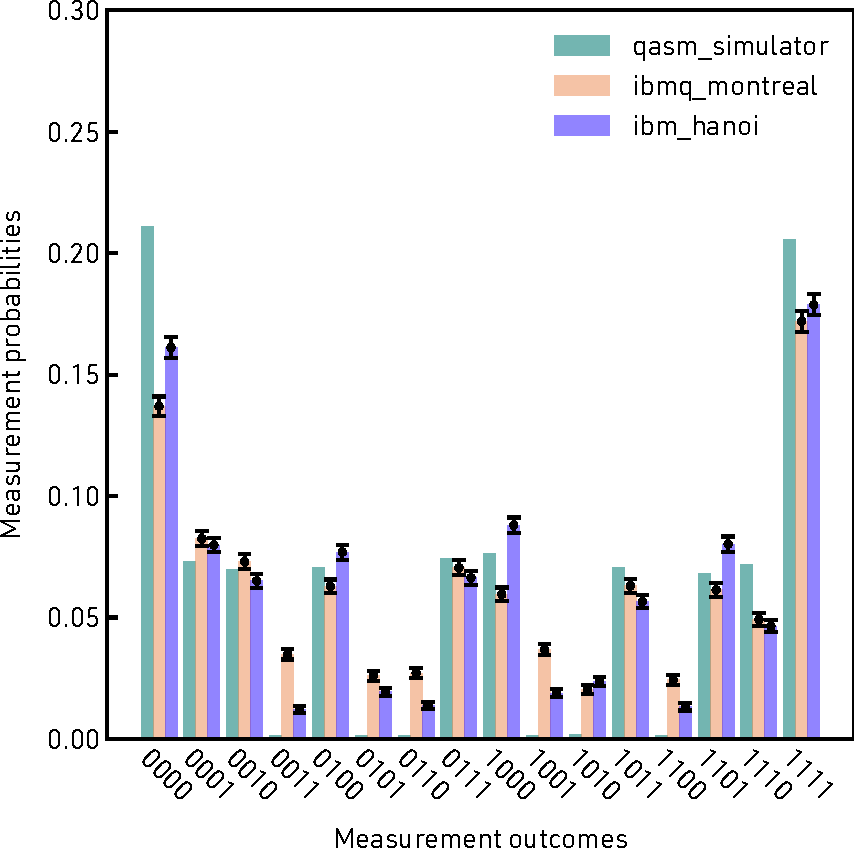
\includegraphics[width=0.86\textwidth]{K14_outcomes}
    \caption[Results of the \acs{max-cut} problem for the star graph $K_{1,4}$ on IBM Q processors.][50pt]{Results of the \acs{max-cut} problem for the star graph $K_{1,4}$ on IBM Q processors. The four-qubit circuit in~\protect\refFigureOnly{grover_k14} is used where the qubit for vertex $0$ is not included as described in the main text. On each processor, the circuit was executed ${8192 \times 900}$ times with measurement error mitigation. The error bars represent ${95\%}$ confidence intervals around the mean value of each histogram bin (See~\protect\refSectionOnly{error_bars} of technical~\protect\refAppendixOnly{appendix_A} for details). The simulator probabilities show the ideal case.}
    \labelFigure{K14_outcomes}
\end{figure}

\clearpage
\noindent
Compared to the results in the study~\cite{Satoh_2020}, they represent an improvement as they exceed $0.11$ for the \acs{max-cut} solution. However, the comparison is a bit unfair, as the improvement of the results is probably indicative of the improvement of the capabilities of the IBM Q processors more than anything else, as the study~\cite{Satoh_2020} used earlier processors that could only tolerate lower two-qubit gates in a circuit than the currently reported $30$ two-qubit gate limit for current IBM Q processors~\cite{Gwinner_2020,Zhang_2021}. More importantly, our transpiled circuit uses $6$ more controlled-NOT gates. 

\bigskip
\noindent
We now improve the maximum ideal probability for measuring the \acs{max-cut} by using a further Grover iterate that uses a local diffuser operator as shown in~\refFigureOnly{grover_k14_mod}. The circuit is mapped to a physical device using the same mapping as in~\refFigureOnly{K14_mappings}~\refSubfigureOnly{K14_mod_mapping} as before, with the controlled-NOT gates in the transpiled circuit tallying to $33$. 

\begin{figure}[h]
	\centering
	\resizebox{1.0\textwidth}{!}{%
	\begin{tikzpicture}
		\begin{yquant}[register/separation=4mm]
			qubit {$q_{\idx}$} q[4];


			[this subcircuit box style={draw, dashed, inner ysep=6pt, label=above:$O(\theta_0)$}]
			subcircuit {
				qubit {} q[4];
				box {$R_z(\theta_0)$} q;
			} (q);


			[this subcircuit box style={draw, dashed, inner ysep=6pt, label=above:$D_{4,3}$}]
			subcircuit {
				qubit {} q[3];
				x q[0-2];
				h q[0-2];
				box {$Z$} q[2] | q[0-1];
				h q[0-2];
				x q[0-2];

			} (q[0-2]);

			[this subcircuit box style={draw, dashed, inner ysep=6pt, label=above:$O(\theta_1)$}]
			subcircuit {
				qubit {} q[4];
				box {$R_z(\theta_1)$} q;
			} (q);


			[this subcircuit box style={draw, dashed, inner ysep=6pt, label=above:$D_4$}]
			subcircuit {
				qubit {} q[4];
				x q;
				h q;
				box {$Z$} q[3] | q[0-2];
				h q;
				x q;
			} (q);
			measure q;
		\end{yquant}
	\end{tikzpicture}
	}
	\caption[A circuit diagram for the \acs{max-cut} problem for the star graph $K_{1,4}$ realized on four qubits that uses two Grover iterates improves over the ideal probability of \acs{max-cut} in the study~\cite{Satoh_2020}.]{A circuit diagram for the \acs{max-cut} problem for the star graph $K_{1,4}$ realized on four qubits that uses two Grover iterates improves over the ideal probability of \acs{max-cut} in the study~\cite{Satoh_2020}. Here, one local Grover iterate $G_{4,3}(\theta_0)$ where ${\theta_0\simeq 0.323\pi}$ and a global Grover iterate $G_{4}(\theta_1)$ where ${\theta_1\simeq 0.322\pi}$ yield an ideal probability of observing the \acs{max-cut} outcome close to $0.25$ upon measuring all the qubits in the computational basis.}
	\labelFigure{grover_k14_mod}
\end{figure}

\noindent
We choose the values $\theta_0=\theta_1 \simeq 0.323 \pi$ (more on this choice later ), for this choice the ideal probability of measuring the \acs{max-cut} is close to $0.25$. ~\refFigureOnly{K14_mod_outcomes} shows the readout error mitigated results of measurement outcomes from the two processors. 

\begin{figure}[h]
    \centering
    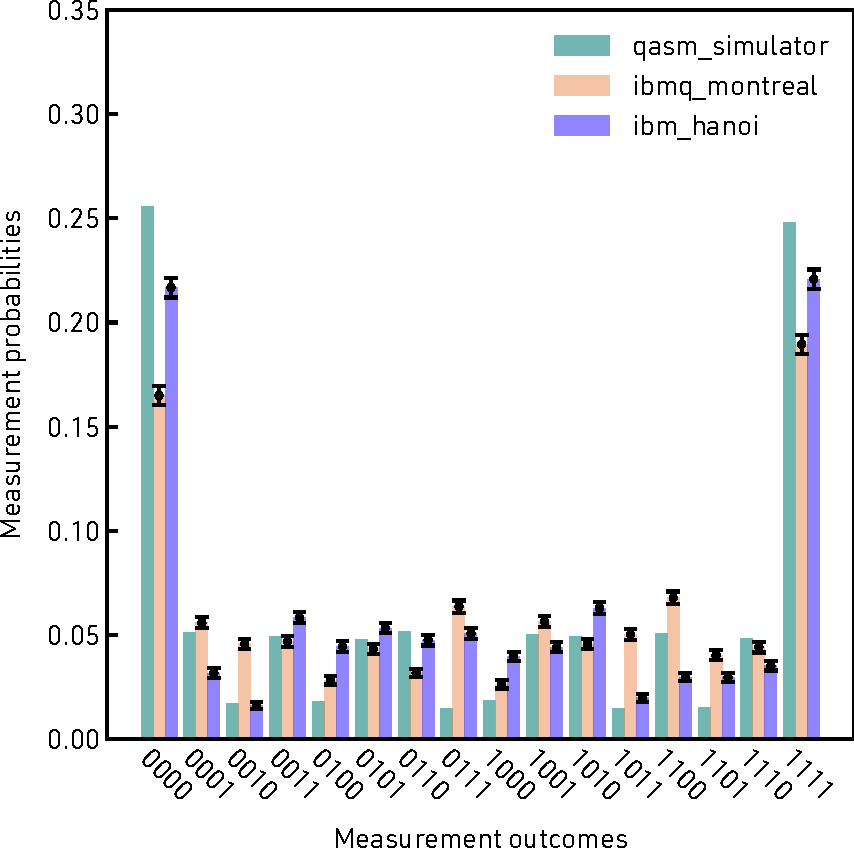
\includegraphics[width=.86\textwidth]{K14_mod_outcomes}
    \caption[Results of the \acs{max-cut} problem with two Grover iterates for the star graph $K_{1,4}$ on IBM Q processors.]{Results of the \acs{max-cut} problem with two Grover iterates for the star graph $K_{1,4}$ on IBM Q processors. The four-qubit circuit in~\protect\refFigureOnly{grover_k14_mod} is used where the qubit for vertex $0$ is not included as described in the main text. On each processor, the circuit was executed ${8192 \times 900}$ times with measurement error mitigation. The error bars represent ${95\%}$ confidence intervals around the mean value of each histogram bin (See~\protect\refSectionOnly{error_bars} of technical~\protect\refAppendixOnly{appendix_A} for details). The simulator probabilities show the ideal case.}
    \labelFigure{K14_mod_outcomes}
\end{figure}

\clearpage
\noindent
The \acs{max-cut} outcome $1111$, and the no-cut outcome $0000$ ($00000$ and $01111$ respectively since virtual vertex $0$ is set to $0$), occur with probability close to $0.16$ and $0.19$, respectively on the \textbf{ibmq\_montreal} processor. And occur with probability close to $0.22$ and $0.22$, respectively on the \textbf{ibm\_hanoi} processor. The Kolmogorov distance between the measured distribution and the ideal distribution is $0.1308$ and $0.1844$ for \textbf{ibmq\_montreal} and \textbf{ibm\_hanoi}, respectively. With an additional local diffuser operator, we have slightly improved over the results in~\refFigureOnly{K14_outcomes}. At the time of writing this thesis, it dawned on the author that the choice of angles $\theta_0$ and $\theta_1$ as $0.323\pi$ for the circuit~\refFigureOnly{grover_k14_mod} do not necessarily achieve the maximum possible ideal probability of measuring the \acs{max-cut} any more. The choice $\theta_0 \simeq 0.301 \pi$ and $\theta_1 \simeq 0.541 \pi$ for the circuit shown in~\refFigureOnly{grover_k14_mod} yields a maximum ideal probability for measuring the \acs{max-cut} close to $0.311$. Interestingly, another revelation that occurred to the author is that the local diffuser operator $D_{4,3}$ in~\refFigureOnly{grover_k14_mod} can be replaced with a smaller local diffuser operator $D_{4,2}$ as shown in~\refFigureOnly{grover_k14_modd}. Choosing the angles $\theta_0$ and $\theta_1$ as $0.359\pi$ and $0.814\pi$, respectively yields a probability of measuring the \acs{max-cut} close to $0.2482$.

\begin{figure}[h]
	\centering
	\resizebox{1.0\textwidth}{!}{%
	\begin{tikzpicture}
		\begin{yquant}[register/separation=4mm]
			qubit {$q_{\idx}$} q[4];


			[this subcircuit box style={draw, dashed, inner ysep=6pt, label=above:$O(\theta_0)$}]
			subcircuit {
				qubit {} q[4];
				box {$R_z(\theta_0)$} q;
			} (q);


			[this subcircuit box style={draw, dashed, inner ysep=6pt, label=above:$D_{4,2}$}]
			subcircuit {
				qubit {} q[2];
				x q[0-1];
				h q[0-1];
				box {$Z$} q[1] | q[0];
				h q[0-1];
				x q[0-1];

			} (q[0-1]);

			[this subcircuit box style={draw, dashed, inner ysep=6pt, label=above:$O(\theta_0)$}]
			subcircuit {
				qubit {} q[4];
				box {$R_z(\theta_1)$} q;
			} (q);


			[this subcircuit box style={draw, dashed, inner ysep=6pt, label=above:$D_4$}]
			subcircuit {
				qubit {} q[4];
				x q;
				h q;
				box {$Z$} q[3] | q[0-2];
				h q;
				x q;
			} (q);
			measure q;
		\end{yquant}
	\end{tikzpicture}
	}
	\caption[A circuit diagram for the \acs{max-cut} problem for the star graph $K_{1,4}$ realized on four qubits that uses two Grover iterates improves over the ideal probability of \acs{max-cut} in the study~\cite{Satoh_2020} even with a smaller local diffuser operator compared to ~\protect\refFigureOnly{grover_k14}.]{A circuit diagram for the \acs{max-cut} problem for the star graph $K_{1,4}$ realized on four qubits that uses two Grover iterates improves over the ideal probability of \acs{max-cut} in the study~\cite{Satoh_2020} even with a smaller local diffuser operator compared to ~\protect\refFigureOnly{grover_k14}. Here one local Grover iterate $G_{4,2}(\theta_0)$ where ${\theta_0 \simeq 0.359\pi}$ and global Grover iterate $G_{4}(\theta_1)$ where ${\theta_1 \simeq 0.814\pi}$ yields an ideal probability of observing the \acs{max-cut} outcome close to $0.2482$ upon measuring all the qubits in the computational basis.}
	\labelFigure{grover_k14_modd}
\end{figure}

\noindent
Unfortunately, the author realized the aforementioned possibilities quite late in their thesis writing when they returned to the \acs{max-cut} problem and could not test the two circuits in shown~\refFigureOnly{grover_k14_mod} and~\refFigureOnly{grover_k14_modd} on the IBM Q processors in time. However, it is not too far-fetched to think that the results would slightly improve over the ones presented here, even more so, for the circuit in~\refFigureOnly{grover_k14_mod}, since it would be transpiled to a circuit with fewer two-qubit gates. This combination of local and global diffuser operators together with a subdivided oracle $O(\theta)$, where the $\theta$ are optimized at each stage to maximize the probability of observing the \acs{max-cut} solution, is an interesting direction for future work in realizing the \acs{max-cut} problem on \acs{NISQ} processors. 


\bigskip
\noindent
However, it is unlikely that such an algorithm can be still considered as Grover's algorithm because we modify the angles of the oracle at each step by classically finding the optimal angles $\theta_i$ for the oracle $O(\theta_i)$ that achieve maximum probability of observing the desired outcome at that step. Such an algorithm is comparable to hybrid quantum/classical algorithms such as the \gls{VQE}~\cite{Peruzzo_2014} and \gls{QAOA}~\cite{Farhi_2014}. In a similar fashion, the aforesaid algorithms seek to prepare some desired $n$-qubit state $\ket{\psi}$ that maximizes/minimizes some objective cost function. In the case of \acs{VQE}, the desired state $\ket{\psi}$ is one that minimizes the expectation value $\expval{H}{\psi}/\ip{\psi}$ with respect to some Hamiltonian $H$. For \acs{QAOA},  $\ket{\psi}$ maximizes some cost function for an optimization problem such as the \acs{max-cut} (see Ref.~\cite{Farhi_2014} details). 

\bigskip
\noindent
For both algorithms at each step, a sequence of gates $U_1(\theta_1)U_2(\theta_2)\cdots U(\theta_n)$ parameterized with tunable parameter(s) $\vec{\theta}$ is applied to the current best approximation of $\ket{\psi}$ after which, a quantum computer evaluates the objective function and the classical computer aids by optimizing the parameters $\vec{\theta}$ for the next evaluation step. For the previously described scheme, the oracle $O(\theta)$ can be viewed as the $U_1(\theta)U_2(\theta)\cdots U(\theta)$ and the objective cost function is $p(\theta)$ from~\refEquationOnly{p_theta}. Recently, such a hybrid quantum/classical approach to Grover's canonical search algorithm has been considered in the study~\cite{Morales_2018}. For a parametrized phase oracle and non-parametrized diffuser (and other), such a hybrid approach achieves a better success probability than Grover's algorithm canonical quantum search for small search space size $N$, asymptotically both algorithms have the same performance~\cite{Morales_2018}.

\subsection{Quantum search in measurement-based quantum computing}
\labelSection{C2_quantum_search_in_measurement_based_quantum_computing}

The experimental demonstrations of Grover's algorithm have also been realized in the context of \gls{MBQC} on graph states. The canonical quantum search algorithm on two qubits has been experimentally realized by different studies thus far~\cite{Walther_2005,Prevedel_2007,Chen_2007,Barz_2012} on a four-qubit graph state. Common among the aforementioned references, is the realization that the canonical quantum search algorithm on two qubits naturally arises as a measurement procedure on a four-qubit box graph state shown in~\refFigureOnly{box_graph}.

\begin{marginfigure}
	\centering
	\tikzfig{graphics/box_graph}
    \caption[Four qubit box graph state realized by first preparing all qubits in the $\ket{+}$, and then applying controlled-$Z$ gates between qubits with edges connecting them.]{Four qubit box graph state realized by first preparing all qubits in the $\ket{+}$, and then applying controlled-$Z$ gates between qubits with edges connecting them.}
	\labelFigure{box_graph}
\end{marginfigure}

\bigskip
\noindent
Recall that in~\acs{MBQC}, gates are simulated by performing measurements on an initially prepared graph state in the equatorial measurement basis $B(\alpha) = \{ \ket{+\alpha},\ket{-\alpha}\}$, where $\ket{\pm \alpha}_j = (\ket{0}_j \pm e^{i\alpha}\ket{1})$. Thus if we measure qubits $0$ and $3$ in the basis $B_0(\alpha)$ and $B_3(\beta)$, respectively. This set of measurements effectively applies the $(X^{m_0} H R_z(\alpha))^{(q_0)} \otimes(X^{m_3} H R_z(\beta))^{(q_3)}CZ_{q_{0}q_{3}}$ on qubits $\ket{q_0}$ and qubit $\ket{q_3}$ of graph state shown in~\refFigureOnly{box_graph}~\footnote{See Ref.\cite{Jozsa_2005,Nielsen_2006,Browne_2016} for detailed descriptions of \acs{MBQC}.}. The values $m_0, m_3 \in \{0,1\}$ denote measurement outcomes of the preceding measurements outcomes where a value of $m_i=0$ or $m_i=1$ indicates that we measured the $\ket{+\alpha}$ or $\ket{-\alpha}$ state, respectively, on qubit $i$. Lastly, we perform the measurement $B(\pi)$ on both qubits $1$ and $2$. 

%p \begin{figure}[h]
% 	\centering
% 	\resizebox{1.0\textwidth}{!}{%
% 	\begin{tikzpicture}
% 		\begin{yquant}[register/separation=4mm]
% 			qubit {$\ket{q_0}=\ket{+}$} q0;
% 			qubit {$\ket{q_1}=\ket{+}$} q1;
% 			qubit {$\ket{q_2}=\ket{+}$} q2;
% 			qubit {$\ket{q_3}=\ket{+}$} q3;

% 			box {$Z$} q1 | q0;
% 			box {$Z$} q2 | q1;
% 			box {$Z$} q3 | q2;
% 			box {$Z$} q3 | q0;


% 			[this subcircuit box style={draw, dashed, inner ysep=6pt, label=above:$B_0(\alpha)$}]
% 			subcircuit {
% 				qubit {} q0;
% 				box {$R_z(\alpha)$} q0;
% 				h q0;
% 				measure q0;
% 			} (q0);

% 			[this subcircuit box style={draw, dashed, inner ysep=6pt, label=below:$B_3(\beta)$}]
% 			subcircuit {
% 				qubit {} q3;
% 				box {$R_z(\beta$)} q3;
% 				h q3;
% 				measure q3;
% 			} (q3);

% 			box {$R_z(\alpha) H X^{m_0}$} q1 | q0;
% 			box {$R_z(\beta) H X^{m_2}$}  q2 | q3;

% 			discard q1;
% 			discard q2;

% 			init {$X^{m_0} H R_z(\alpha) \ket{q_0}$} q1;
% 			init {$X^{m_3}  H R_z(\beta) \ket{q_3}$} q2;

% 			box {$R_z(\pi)$} q1;
% 			h q1;

% 			box {$R_z(\pi)$} q2;
% 			h q2;

% 			measure q1;
% 			measure q2;
% 		\end{yquant}
% 	\end{tikzpicture}
% 	}
% 	\caption[A circuit diagram equivalent of the measurement procedure on a four qubit graph state realizes Grover's two-qubit quantum search algorithm.]{A circuit diagram equivalent of the measurement procedure on a four qubit graph state realizes Grover's two-qubit quantum search algorithm; the circuit begins by measuring qubits $0$ and $3$ in the basis $B(\alpha)$ and $B(\beta)$ respectively, which effectively applies $X^{m_a} H R_z(\theta)$ to each qubit, where $m_a$ is the measurement outcome on qubit $a$. After which, the resultant joint state on qubit $0$ and $3$ is teleported to qubit $1$ and $2$, respectively. The final round of measurements is on qubits $1$ and $2$, which we both measure in the basis $B(\pi)$.}
% 	\labelFigure{4q_graph_state_circ}
% \end{figure}

\bigskip
\noindent
It is useful to write $X^{m_a} H R_z(\theta)$ as $H Z^{m_a} R_z(\theta)$ where we use the identity $X H = H Z$. From this, the effective two-qubit state after the above measurement procedure that resides on qubits $2$ and $3$ is equivalent to the circuit diagram shown in~\refFigureOnly{2q_grover} in the quantum circuit model. The aforementioned circuit realizes Grover quantum search algorithm on two qubits for an appropriate choice of the angles $\alpha$ and $\beta$, in the case where $m_0=m_3=0$. For the choice of angles $(\alpha, \beta) = (-\pi,-\pi), (-\pi, 0), (0,-\pi)$ and $(0,0)$, the phase oracle puts a negative sign on the amplitude of the state $\ket{00}, \ket{01}, \ket{10}$ and $\ket{11}$, respectively. For any combination of $m_0,m_3$, the above circuit still realizes Grover's algorithm with an appropriate reinterpretation of the measurement outcomes. The interested reader may refer to section~\refSectionOnly{grover_equivalence_mbqc} of the technical~\refAppendixOnly{appendix_B} for more details.

\begin{figure}[h]
	\centering
	\begin{tikzpicture}
		\begin{yquant}[register/separation=4mm]
			qubit {$\ket{q_0}=\ket{+}$} q0;
			qubit {$\ket{q_1}=\ket{+}$} q1;

			[this subcircuit box style={draw, dashed, inner ysep=6pt, label=above:Phase oracle}]
			subcircuit {
 				qubit {} q0;
 				qubit {} q1;

 				box {$Z$} q1 | q0;
 				box {$R_z(\alpha)$} q0;
 				box {$R_z(\beta)$} q1;
				box {$Z^{m_0}$} q0;
				box {$Z^{m_3}$} q1;
			} (q0, q1);

			[this subcircuit box style={draw, dashed, inner ysep=6pt, label=above:Diffuser}]
			subcircuit {
				qubit {} q0;
				qubit {} q1;

				h q0, q1;
				box {$Z$} q1 | q0;
				z q0;
				z q1;
				h q0, q1;
			} (q0, q1);

			measure q0, q1;
		\end{yquant}
	\end{tikzpicture}
	\caption[A circuit diagram equivalent of the remaining two qubit after the four-qubit measurement procedure descibed in the main text.]{A circuit diagram equivalent of the remaining two qubit after the four-qubit measurement procedure described in the main text; the resultant circuit realizes Grover's algorithm for two qubits with the appropriate choice of angles $\alpha$ and $\beta$. For ${(\alpha, \beta) = (-\pi,-\pi), (-\pi, 0), (0,-\pi)}$ and $(0,0)$ the circuit finds the target $\ket{00}, \ket{01}, \ket{10}$ and $\ket{11}$ respectively.}
	\labelFigure{2q_grover}
\end{figure}

\clearpage
\noindent
In my honours studies, we realized the above measurement-based Grover's algorithm for two qubits successfully on IBM Q processors. Additionally, we were able to realize a measurement-based Grover's algorithm for two qubits on a graph state with one fewer edge, thus one less two-qubit gate in its state preparation. The original four-qubit graph state and the latter graph state belong to the same \acs{LU}-equivalence class~\cite{Hein_2004, Nest_2004}. The local unitaries relating the two states can be derived by successive applications of the edge local complementation rule~\cite{Hein_2004,Nest_2004}. For the interested reader, the missing details are filled in sections~\refSectionOnly{grover_equivalence_mbqc} and ~\refSectionOnly{4q_lu_equiv_meas_proc} of the technical~\refAppendixOnly{appendix_B}.

\bigskip
\noindent
Hence, we considered the next natural step; whether it would be possible to realize a measurement-based Grover's algorithm for three qubits. The initial hurdle was that the quantum circuit model equivalent of Grover's algorithm on three qubits does not naturally arise as a measurement procedure on any well known graph state unlike the case for two qubits, as far as we are aware. An unsophisticated way to circumvent this hurdle is to look for measurement-based implementations of the various gates in the quantum circuit model of Grover's algorithm for three qubits, and thus by constructing the measurement-based equivalent of each gate in the circuit and linking them together, one can realize the entire circuit as a measurement-based procedure.

\begin{marginfigure}
	\centering
    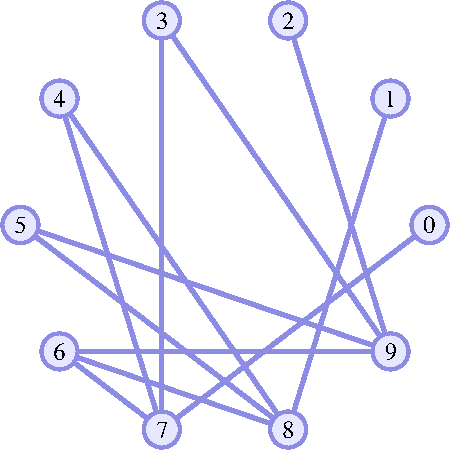
\includegraphics[width=0.65\textwidth]{10q_graph_state}
    \caption[Ten-qubit graph state used as a resource for realizing a measurement-based controlled-controlled-$Z$ gate.]{Ten-qubit graph state used as a resource for realizing a measurement-based three-qubit Toffoli gate. Qubits $0,1,2,6$ are measured in the $H B(\pi/4)$ basis and qubits $3,4,5$ in the $H B(\pi/4)$ basis, which realizes a controlled-controlled-$Z$ gate up to measurement outcome byproducts acting on the inputs in qubits $7,8$ and $9$ as two control and target qubits, respectively.}
	\labelFigure{10q_graph_state}
\end{marginfigure}

\noindent
As we have seen earlier, the $n$-qubit $C^{n-1}[Z]$, in this case, a controlled-controlled-$Z$ gate constitutes the most resourceful part in Grover's algorithm, appearing in both the phase oracle and diffuser operators. The canonical measurement-based controlled-controlled-$Z$ due to Browne and Briegel~\cite{Browne_2016} can be realized on a graph state of ten qubits. The measurement-based controlled-controlled-$Z$ gate is a special case of a general result from the aforementioned reference, any $n$-qubit unitary operator diagonal in the computational basis of the form~\cite{Browne_2016}


\begin{align}
	U_n &= \displaystyle\prod_{\vec{m}} \exp(i \frac{\theta_{\vec{m}}}{2} (Z_1)^{m_1} \otimes (Z_2)^{m_2} \otimes \cdots \otimes (Z_n)^{m_n} ), \nonumber \\
	&= \exp(\frac{i}{2}\displaystyle\sum_{\vec{m}} \theta_{\vec{m}} (Z_1)^{m_1} \otimes (Z_2)^{m_2} \otimes \cdots \otimes (Z_n)^{m_n}),
\end{align}

\noindent
where $m_j \in \{0, 1\}$ and $Z_j$ is the Pauli $Z$ operator acting on qubit $j$. The sum is performed over all possible bit strings of length $n$. From the above form, the controlled-controlled-$Z$ gate is realized by the following choice of angles

\begin{align}
	\theta_{000} = 0, \theta_{001} = -\frac{\pi}{4}, \theta_{010} = -\frac{\pi}{4}, \theta_{011} = \frac{\pi}{4}, \nonumber \\
	\theta_{100} = -\frac{\pi}{4}, \theta_{101} = \frac{\pi}{4}, \theta_{110} = \frac{\pi}{4}, \theta_{111} = -\frac{\pi}{4}.
\end{align}

\noindent
The ten-qubit graph state that realizes the three-qubit Toffoli gate is shown in~\refFigureOnly{10q_graph_state}. The input qubits $7,8$ and $9$ can be prepared in any single-qubit state rather than strictly $\ket{+}$ since qubits $7,8$ and $9$ are designated as input controls and target qubits, respectively, for the \acs{MBQC} controlled-controlled-$Z$ gate. Thus, the procedure to realize a controlled-controlled-$Z$ gate with input qubits $\ket{c_1}, \ket{c_2}, \ket{t}$ as follows: (i) Prepare inputs $\ket{c_1}, \ket{c_2}, \ket{t}$ to any state of our choosing, the rest of the qubits are prepared in the $\ket{+}$, and we perform controlled-$Z$ gates on qubits connected by an edge in~\refFigureOnly{10q_graph_state}. (ii) perform the projective measurements of the $H B(\theta) = \cos{\theta/2}\ket{0}\pm \sin{\theta/2}\ket{1}$, with $\theta=\pi/4$ for qubits $0, 1, 2, 6$ and $\theta=-\pi/4$ for qubits $3,4,5$, respectively~\cite{Browne_2016}. 

\noindent
The above measurement procedure realizes a three qubit controlled-controlled-$Z$ gates acting on the inputs $c_1, c_2, t$ and output of the gate residing on qubits $7,8$ and $9$, up to the byproduct Pauli operators that arise from the measurement outcomes.

\begin{align}
	(Z^{m_0+ m_3 + m_4+m_6})^{(7)} \otimes (Z^{m_1+ m_4+m_5+m_6})^{(8)} \otimes (Z^{m_2}Z^{m_3}Z^{m_5}Z^{m_6})^{(8)},
\end{align}

\noindent
where $m_i \in \{0, 1\}$ is an outcome from the aforementioned measurement procedure on qubit $i$, and the byproducts act on qubits $7,8$ and $9$, respectively.

\begin{marginfigure}
	\centering
	\tikzfig{graphics/10q_mapping}
    \caption[Physical device ten-qubit mapping for the ten-qubit graph state in~\protect\refFigureOnly{10q_graph_state}.]{Physical device ten-qubit mapping for the ten-qubit graph state in~\protect\refFigureOnly{10q_graph_state}; each labeled node in the aforesaid is mapped to the corresponding labeled qubit in this figure.}
	\labelFigure{10q_mapping}
\end{marginfigure}

\bigskip
\noindent
In implementing the described measurement-based controlled-controlled-$Z$ gate on IBM Q, we begin by mapping the graph state to the qubits of a physical device. The graph state in~\refFigureOnly{10q_graph_state} is highly connected, and no physical device exists with such a topology. Thus, we choose to map qubits that have the most connections to the physical qubits that have most connections on the physical device; in~\refFigureOnly{10q_graph_state} the qubits $7,8$ and $9$ have the most edges. We show a physical device mapping in~\refFigureOnly{10q_mapping}, which results in $60$ controlled-NOT gates for the transpiled circuit. Such a number of two-qubits gates in circuit is well-beyond the $30$ two-qubit gate count limit~\cite{Gwinner_2020}, nonetheless we tested the measurement-based controlled-controlled-$Z$ gate by preparing the qubits $7,8$ and $9$ in various input states, and subsequently performed quantum state tomography to recover the corresponding output states, and then measured the state fidelity of each of the recovered output states against a set of expected output states. From these measurements, we are able to construct a truth table for the controlled-controlled-$Z$ gate for various input and output states, this is shown in~\refFigureOnly{MBQC_toff}. As seen can be seen by the naked eye, the discrepancies between the ideal truth tables and measured truth tables on the \textbf{ibmq\_montreal} and \textbf{ibmq\_mumbai} are quite conspicuous.  We show the greatest element difference between the ideal and the measured truth tables for both processors in~\refTableOnly{element_diff}. The fourth truth table shows the smallest value among the truth tables, which corroborates with the visual representation of the fourth truth table in~\refFigureOnly{MBQC_toff}, as it bears somewhat of an resemblance to the corresponding ideal truth table. 

\begin{table}[h!]
	\centering
	\labelTable{element_diff}
	\caption[The maximum element difference between a measure truth table and corresponding ideal truth table for the truth tables of measurement-based controlled-controlled-$Z$ in~\protect\refFigureOnly{MBQC_toff}.]{The maximum element difference between a measured truth table and corresponding ideal truth table for the truth tables of measurement-based controlled-controlled-$Z$ in~\protect\refFigureOnly{MBQC_toff}. }
	\begin{tabular}{ccc}
		\toprule
		 Figures & $\mathcal{E}_\text{mumbai} - \mathcal{E}_\text{ideal}$ & $\mathcal{E}_\text{montreal} - \mathcal{E}_\text{ideal}$ \\
		\toprule
		(b) and (c)  & $0.427$      &  $0.395$ \\
		(e) and (f)  & $0.401$      &  $0.336$ \\ 
		(h) and (i)  & $0.435$      &  $0.353$ \\
		(k) and (l)  & $0.308$      &  $0.268$ \\
		\toprule
	\end{tabular}
\end{table}

\bigskip
\noindent
Similar to the case for the four-qubit graph realizing Grover's algorithm for two qubits, we can hope to reduce the number of controlled-$Z$ operations we have to apply to create the ten-qubit graph state shown in~\refFigureOnly{10q_graph_state} by finding an \acs{LU}-equivalent graph state with fewer edges. However, it turns out that the graph state in~\refFigureOnly{10q_graph_state} corresponds to the one with the least number of edges in its \acs{LU}-equivalence class.  See the technical appendix~\refAppendixOnly{appendix_B} for details. Thus at the present moment a measurement-based implementation of a controlled-controlled-$Z$ is beyond the reach of current \acs{NISQ} processors. Which subsequently also puts realization of a measurement-based Grover's algorithm for three qubits beyond reach, since at least two controlled-controlled-$Z$ and a few single qubit gates are required to realize Grover's quantum search algorithm for three qubits.

\clearpage

\begin{figure*}[t!]
    \centering
	\subfloat[]
	{
		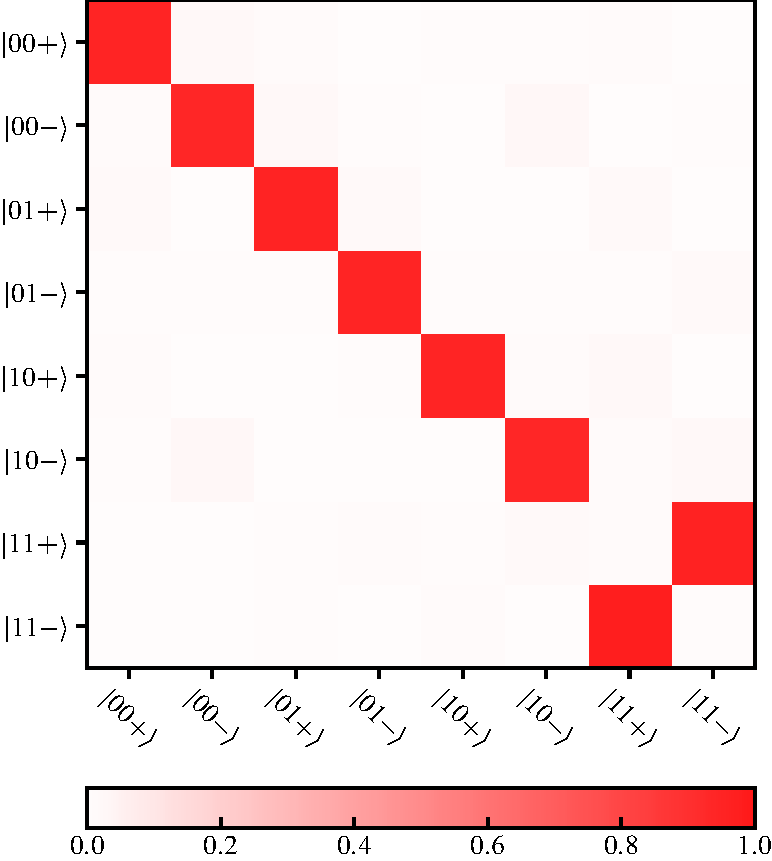
\includegraphics[width=0.33\linewidth]{MBQC_toff_ideal_k0}
	} 
	\subfloat[]
	{
		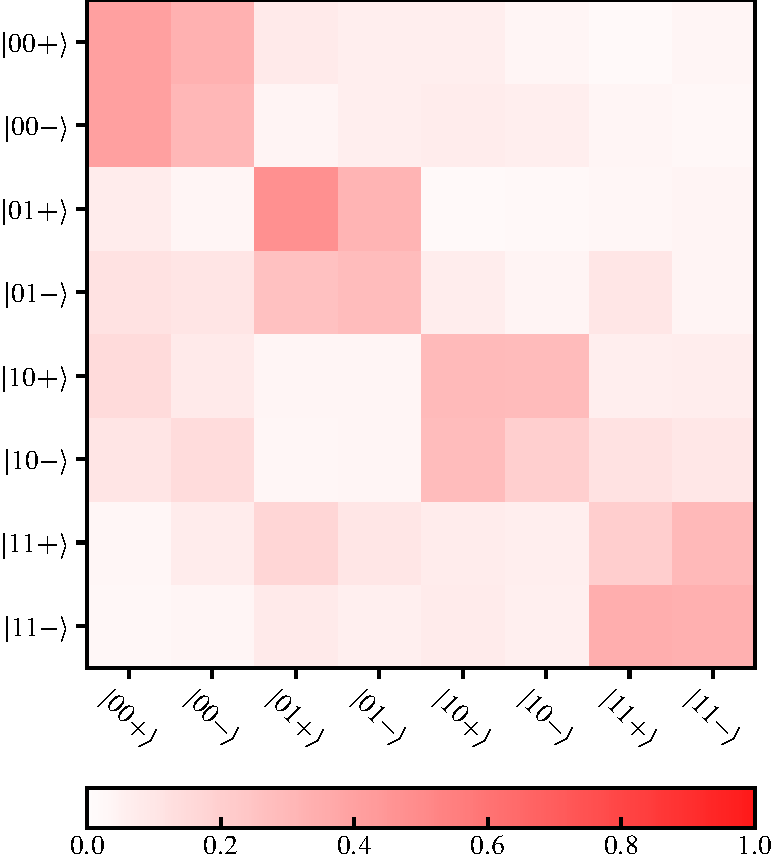
\includegraphics[width=0.33\linewidth]{MBQC_toff_montreal_k0}
	}
	\subfloat[]
	{
		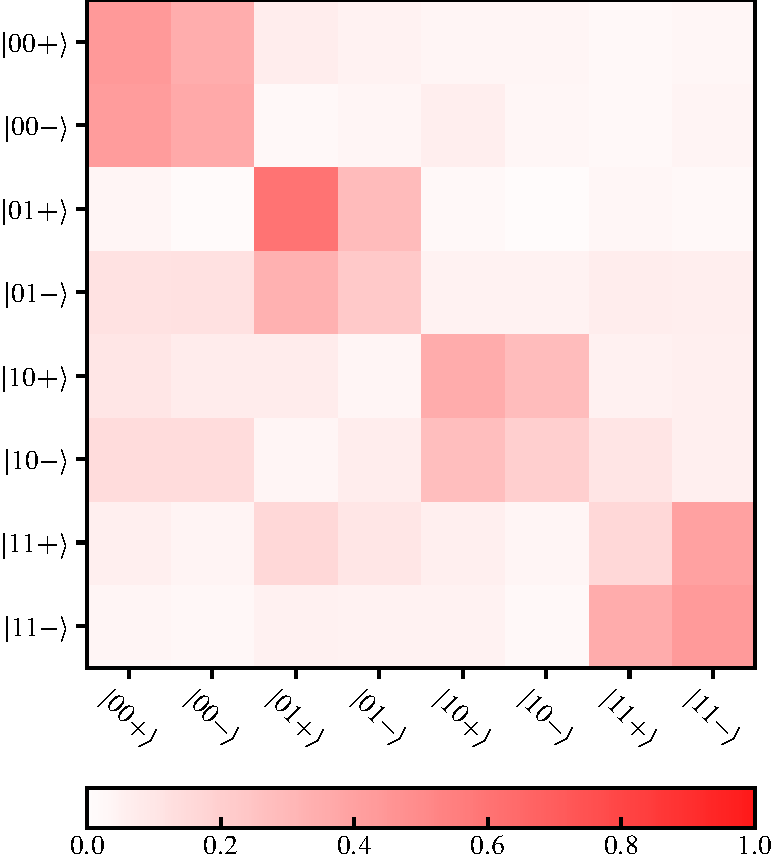
\includegraphics[width=0.33\linewidth]{MBQC_toff_mumbai_k0}
	} \\
	\subfloat[]
	{
		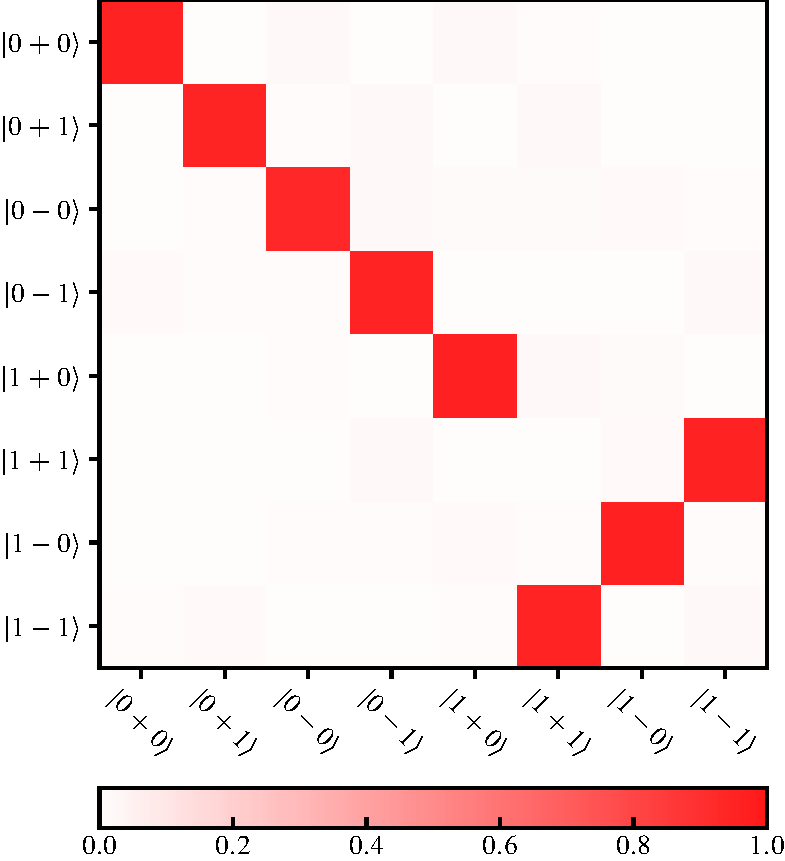
\includegraphics[width=0.33\linewidth]{MBQC_toff_ideal_k1}
	} 
	\subfloat[]
	{
		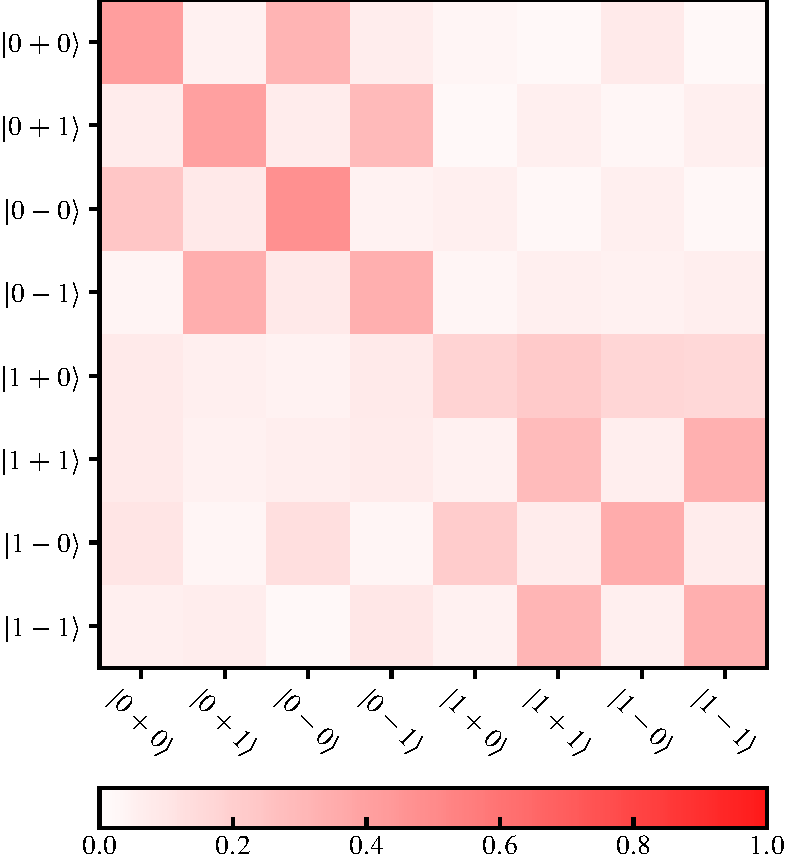
\includegraphics[width=0.33\linewidth]{MBQC_toff_montreal_k1}
	}
	\subfloat[]
	{
		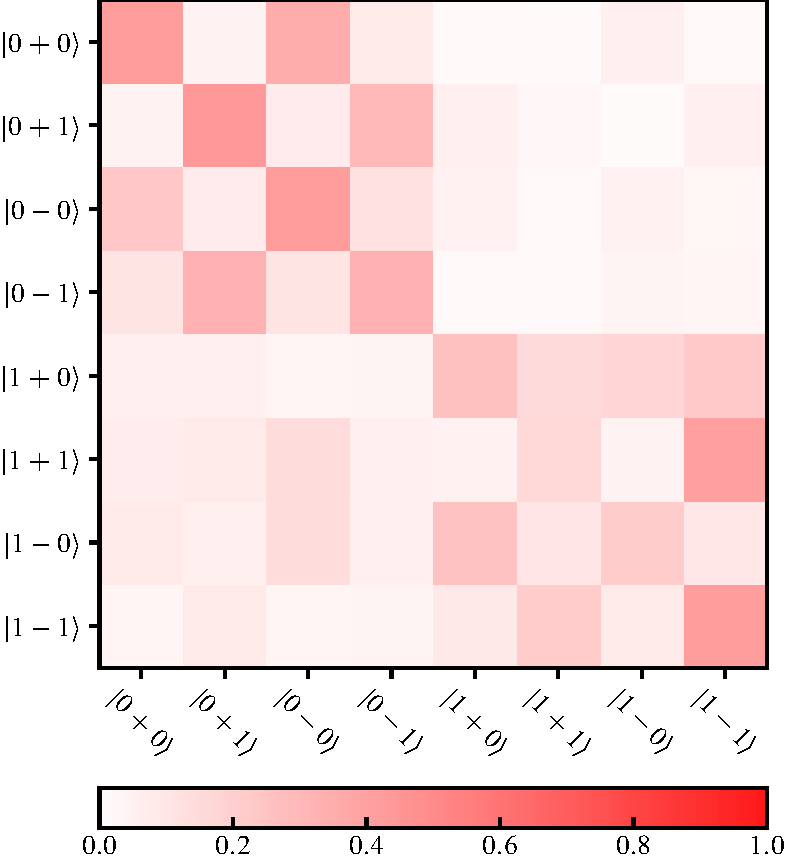
\includegraphics[width=0.33\linewidth]{MBQC_toff_mumbai_k1}
	}  \\
	\subfloat[]
	{
		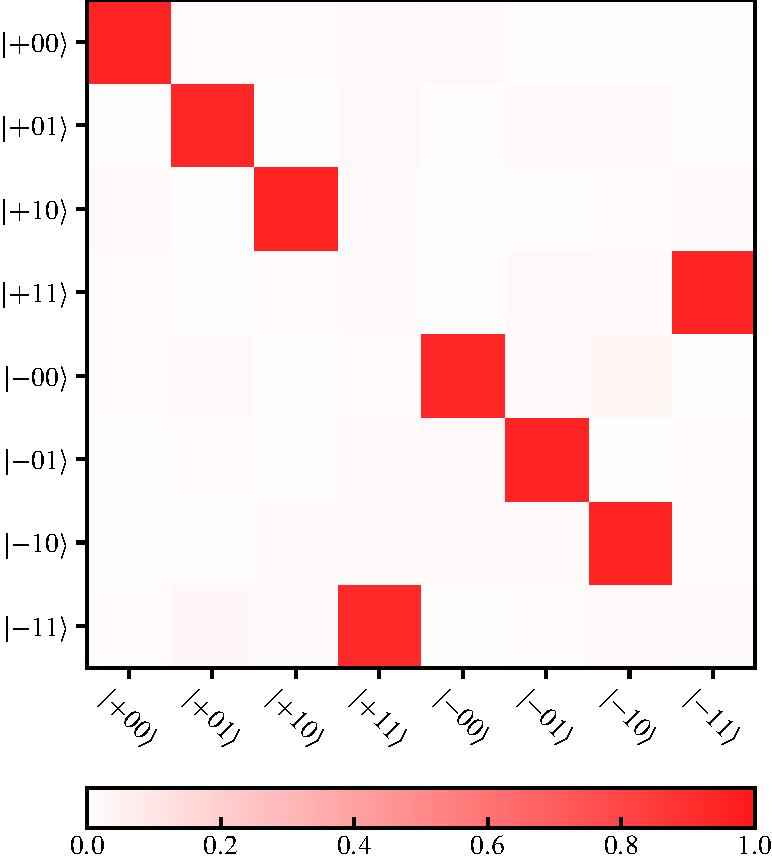
\includegraphics[width=0.33\linewidth]{MBQC_toff_ideal_k2}
	} 
	\subfloat[]
	{
		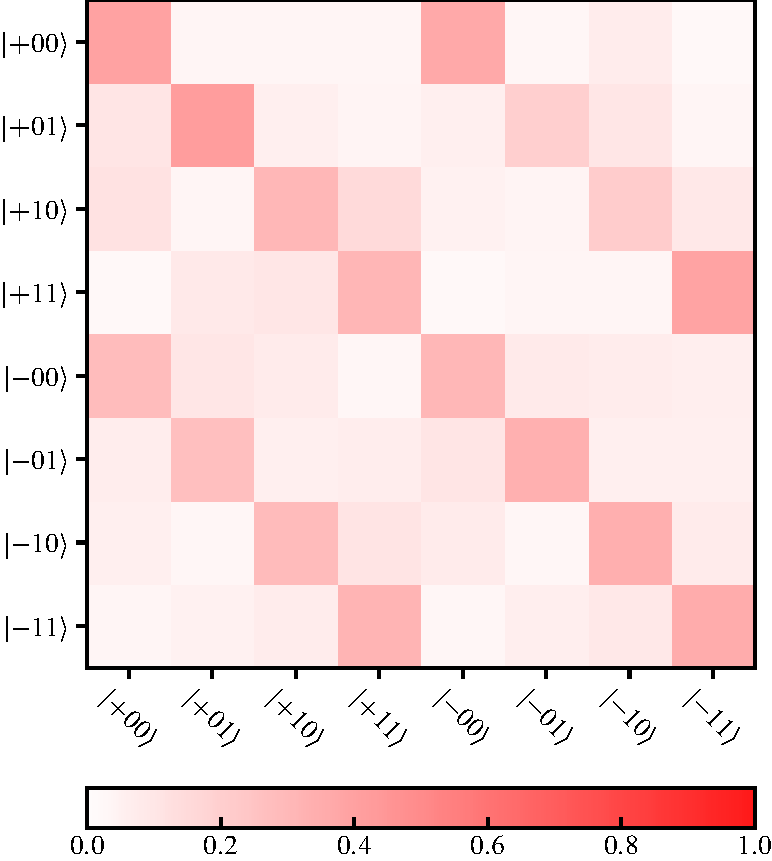
\includegraphics[width=0.33\linewidth]{MBQC_toff_montreal_k2}
	}
	\subfloat[]
	{
		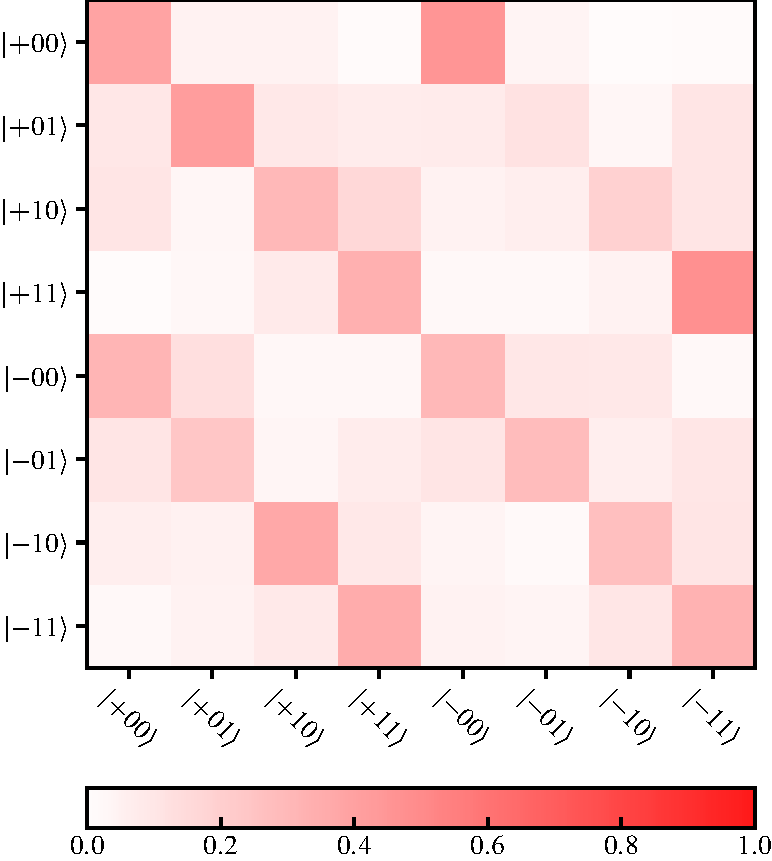
\includegraphics[width=0.33\linewidth]{MBQC_toff_mumbai_k2}
	}
\end{figure*}
\mbox{}
\vfill
\begin{figure*}[t!]
	\setcounter{subfigure}{9}
	\subfloat[]
	{
		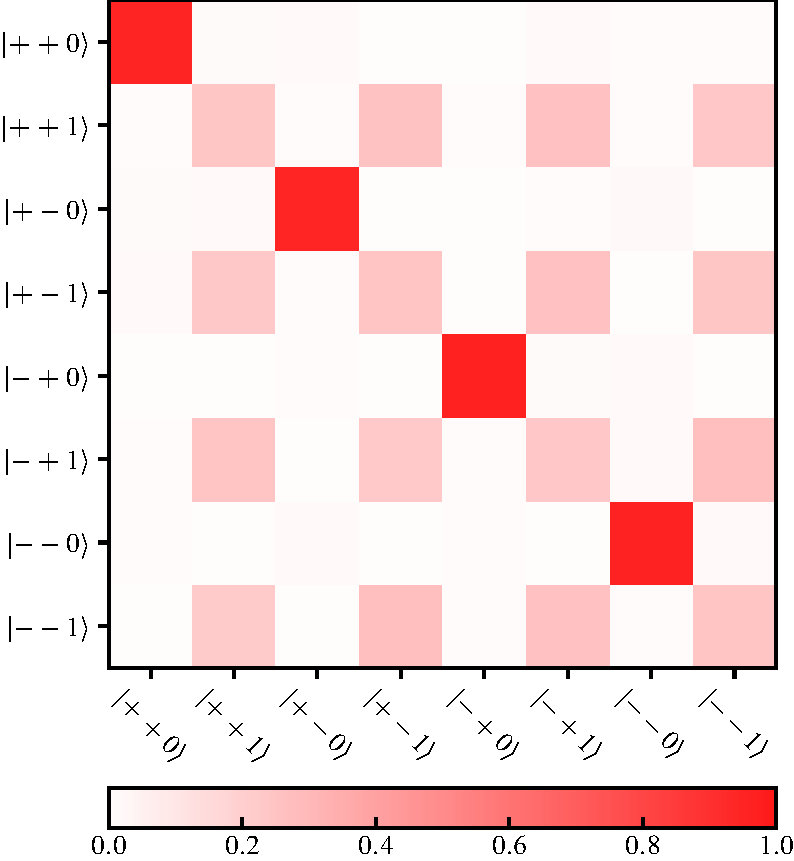
\includegraphics[width=0.33\linewidth]{MBQC_toff_ideal_k3}
	} 
	\subfloat[]
	{
		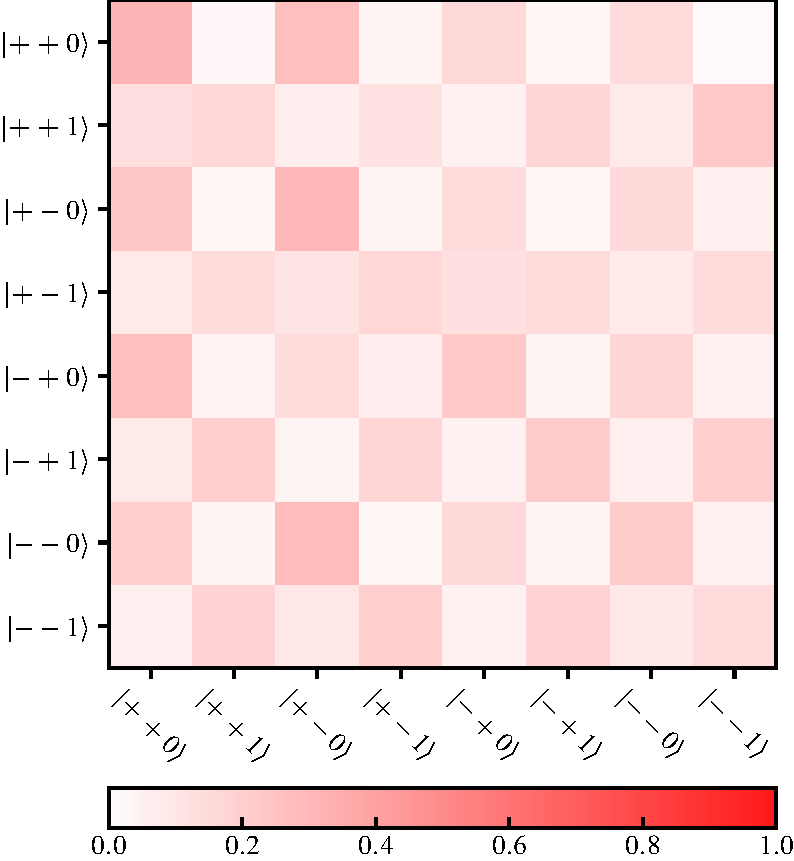
\includegraphics[width=0.33\linewidth]{MBQC_toff_montreal_k3}
	}
	\subfloat[]
	{
		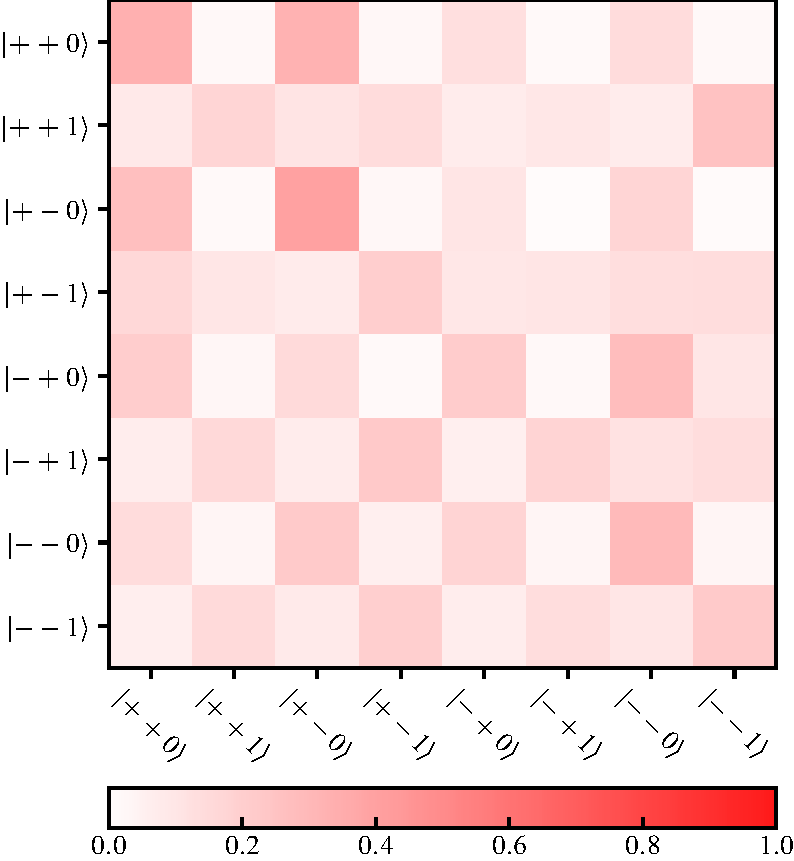
\includegraphics[width=0.33\linewidth]{MBQC_toff_mumbai_k3}
	}
	\caption[Various truth tables for the measurement-based three-qubit controlled-controlled-$Z$ gate.]{Various truth tables for the measurement-based three-qubit controlled-controlled-$Z$ gate. Three figures in each row show a single truth table showing the ideal truth table and measured truth tables from the \textbf{ibmq\_montreal} processor and the measured truth tables from \textbf{ibmq\_mumbai} processor, respectively. When performing the state tomography on the outputs of the gate, we only consider where all the outcomes on the measured qubits are $0$, resulting in no byproducts. \textbf{(a, d, g, j)} Ideal truth tables. \textbf{(b,e,h,k)} Measured truth tables from the processor \textbf{ibmq\_montreal}. \textbf{(c, f, i, l)} Measured truth tables from the processor \textbf{ibmq\_mumbai}.}
	\labelFigure{MBQC_toff}
\end{figure*}


\section{Concluding remarks}
\labelSection{C2_concluding_remarks}

\noindent
 In this chapter, we first began by describing the canonical quantum search algorithm, which assumes no \emph{a priori} knowledge about the structure of the search problem. Such a quantum search algorithm achieves a quadratic speedup over an exhaustive classical search~\cite{Grover_1997}. We also described a variant of the quantum search algorithm called the partial search quantum algorithm, which trades accuracy for speed by finding a partial bit string or target block to which the target element belongs rather than the target element itself~\cite{Grover_2005}. With regards to practicality, especially on \acs{NISQ} processors, the appealing feature of the quantum partial search algorithms in comparison to the canonical quantum search is that they are economical in the number of elementary gates and algorithmic steps they use, albeit the above advantage comes at the expense of accuracy. This realization prompted a large corpus of work interested in realizing small-scale demonstrations of the quantum search algorithm for four qubits and beyond, by reducing the number of elementary operations, particularly two-qubit gates, in quantum search algorithms.

 \bigskip
 \noindent
 Two important theoretical results along these lines were the depth-optimization of the quantum search algorithm, and multi-stage quantum search~\cite{Zhang_2020}, which both place an emphasis on and try to circumvent one of the foremost pressing limitations of \acs{NISQ} processors; short periods of time over which \acs{NISQ} can maintain quantum coherence. The depth-optimized quantum search algorithm optimizes circuit depth of the quantum search algorithm, and hence the algorithmic (proxy) time spent on the processor. The multi-stage quantum search takes this a further step, by breaking up the quantum search algorithm into smaller stages. Each stage performs a smaller quantum search for a substring of the target element at a time, and is executed by a reinitialized circuit. The great advantage of the multi-stage quantum search is that it splits circuits (which would require long coherence times for reliable execution) into smaller circuits that perform the quantum search stage by stage, recovering the target element substring by string, which then reduces the time over which the qubits in each circuit must remain coherent for a reliable execution of the quantum search algorithm, since these qubits are reinitialized at each stage.

\clearpage
\noindent
Studies in such a direction, eventually led to the first realization of a four-qubit quantum search algorithm on IBM Q processors~\cite{Gwinner_2020}. The aforesaid study follows suite in finding ways to circumvent the limitations of \acs{NISQ} processors; by designing multi-qubit gates such as the controlled-$Z$ and controlled-controlled-$Z$ in a manner that is suitable for physical quantum processors with limited connectivity between their physical qubits. Similarly, Ref.~\cite{Zhang_2021} experimentally realized an improved a four-qubit quantum search algorithm through incorporating the methods in~\cite{Zhang_2020} on IBM Q processors. The study in Ref.~\cite{Zhang_2021} also reported an inconclusive five-qubit quantum search algorithm with a success probability comparable to a classical search. Lastly, an application of Grover's algorithm to the \acs{max-cut} problem was studied by Ref.~\cite{Satoh_2020} successfully implementing a proof-of-concept demonstration on IBM Q processors for sparse graphs by proposing a design for a low-depth subdivided phase oracle that assigns a large phase shift to target outcomes and compared to non-target elements. Alas, the advantage for such a demonstration over a classical algorithm was not proved. Nonetheless, our marginal contribution is an adaptation that improves over the theoretical and measured success probability for the \acs{max-cut} by way of an additional shallow depth iteration of the proposed algorithm. Furthermore, we found that if we vary and optimize the phases imparted by the oracle to between iterations to maximize the probability of obtaining the \acs{max-cut} outcome, we can further increase the theoretical success probability for our contributed adaptation. However, it is not clear whether such an adaptation can be still considered as Grover's algorithm; it is comparable to hybrid quantum classical algorithms~\cite{Farhi_2014,Peruzzo_2014,Morales_2018}.

\bigskip
\noindent
Prompted by the success during my Honours studies of a measurement-based Grover's quantum algorithm for two-qubits, we attempted to realize a measurement-based Grover's algorithm for three qubits. We found that, due to the large number of qubits ($10$) and controlled-NOT gates (>$60$) required for simulating a measurement-based controlled-controlled-$Z$ gate on IBM Q processors, the output of the controlled-controlled-$Z$ gate for various truth tables is comparable to uniform noise. Hence, the realization of a three-qubit measurement-based Grover's algorithm is somewhat out of reach for these processors; the situation is even more bleak when we consider that Grover's algorithm for three-qubits requires at least two such gates (one for the phase oracle and another for a diffuser operator) and a few single qubits, which must linked together somehow to realize the full measurement-based quantum search algorithm for three qubits.


\bigskip
\noindent
Another measurement-based implementation of a controlled-controlled-$Z$ (or controlled-controlled-NOT) gate is due to Tame~\etal~\cite{Tame_2009}, which realizes a controlled-controlled-$Z$ gate on a graph state of $8$ qubits. For the eight-qubit graph state in Ref.~\cite{Tame_2009}, some edges between the qubits are created in the usual way by applying a controlled-$Z$ gate between qubits connected by an edge. While other edges are created with a controlled-$R_z(\theta)$ gate for a particular choice of $\theta$,  the standard controlled-$Z$ gate corresponds to $\theta=\pi$. Edges created in this way are called weighted edges, and the angle $\theta$ for such an edge is said to be the weight of that edge. A graph state with edges is said to be a weighted graph~\cite{Tame_2009}. The eight-qubit weighted graph state that realizes a measurement-based controlled-controlled-$Z$ in Ref.~\cite{Tame_2009} has one weighted edge, with a weight $\theta=\pi/2$ and the rest of edges have weight $\theta=\pi$ (corresponds to controlled-$Z$ gate). However, such a measurement-based gate is not yet suitable for IBM Q processors as it requires real-time adaptive measurements for the realized controlled-controlled-$Z$ gate to be deterministic. 

\clearpage
\noindent
As of Nov 2020, IBM's quantum processors do not yet support real-time classical conditionals necessary for the implementation of the adaptive measurements. Alas, in the future once the capability of performing real-time classical conditionals is added, it is not fully clear whether such a measurement-based controlled-controlled-$Z$ gate would offer a significant improvement on \acs{NISQ} processors over the one in Ref.~\cite{Browne_2016}, since the number of qubits and two-qubit gates for the two gates are comparable ($8$ \emph{versus} $10$ qubits , $1$1 \emph{versus} $12$ two-qubits gates, respectively).
